\documentclass[a4paper,11pt]{article}

\usepackage{fullpage}
\usepackage{color}
\usepackage{hyperref}
\usepackage{amsmath}
\usepackage{amssymb}
\usepackage{tikz}
\usepackage{tabularx}
\usepackage{booktabs}
\usepackage{amsmath}
\usepackage{multirow}
\usepackage{layouts}
\usepackage{array}
\usepackage{pgf}
\usepackage{tikz}

\usepackage{amssymb}
\usepackage{graphics}
\usepackage{fancyhdr}
\usepackage{eucal}
\usepackage{ifthen}
\usepackage{ifpdf}
\usepackage{lmodern}
\usepackage{amsthm}
\usepackage{catoptions} % For \Autoref


\usetikzlibrary{positioning}

\hypersetup{
  colorlinks,%
    citecolor=black,%
    filecolor=black,%
    linkcolor=black,%
    urlcolor=mygreylink     % can put red here to visualize the links
}

\definecolor{hlcolor}{rgb}{1, 0, 0}
\definecolor{mygrey}{gray}{.85}
\definecolor{mygreylink}{gray}{.30}
\textheight=8.6in
\raggedbottom
\addtolength{\oddsidemargin}{-0.375in}
\addtolength{\evensidemargin}{0.375in}
\addtolength{\textwidth}{0.5in}
\addtolength{\topmargin}{-.375in}
\addtolength{\textheight}{0.75in}


\newcommand{\resheading}[1]{{\large \colorbox{mygrey}{\begin{minipage}{\textwidth}{\textbf{#1 \vphantom{p\^{E}}}}\end{minipage}}}}

\newcommand{\mywebheader}{
  \begin{tabular}{@{}p{5in}p{4in}}
  {\resheading{Assignment 2: Single Agent Learning}} & {\Large 5 October, 2012}\\\vspace{0.2cm}
  \end{tabular}}

\begin{document}


\begin{center}
{\LARGE \textbf{Autonomous Agents}}\\ [1em]
\end{center}
\mywebheader

\begin{center}
{\Large By:} \\ \vspace{0.1cm}
{\Large Paris Mavromoustakos} \\  \vspace{0.1cm}
{\Large Georgios Methenitis} \\ \vspace{0.1cm}
{\Large Patrick de Kok} \\ \vspace{0.1cm}
{\Large Marios Tzakris}
\end{center}




\section*{Introduction}

In this assignment, we implement the learning scenario: the transition function is unknown to the agents, and so is the reward function. We have implemented several model-based algorithms, which give agents the ability to learn high-reward %maybe a bit inprecise? Patrick
policies while ignoring the model.  

Our code is based on the code handed in for the previous assignment, where we have solved the same problem in a planning setting.  Moreover, we have explicitly used the 21 statespace environment representation which reduced our algorithms' runtime on the previous assignment.


\section*{Exercise 1}

For this first exercise, we have implemented the Q-Learning algorithm with $\epsilon$-greedy action selection, as described in chapter 6, section 5 of the Sutton and Barto book.

On each iteration of this algorithm, we chose an action $a$ of state $s$, and observed the next state and reward we got from it. Then, we updated the Q-learning table according to the following update rule:  

\begin{align*}
  Q(s,a) \leftarrow  Q(s,a) + \alpha \left[ r + \gamma  \max_{a'} Q(s',a') - Q(s,a)\right]
\end{align*}

In this update rule, $Q(s,a)$ represents the value of the state-action pairs based on the previous iteration, while $Q(s',a')$ represents the observed state and possible actions, after action a is chosen. $Q(s,a)$ could be written as $Q(s_t,a_t)$ and $Q(s',a')$ as $Q(s_{t+1}, a_{t+1})$.

$\alpha$ represents the algorithm's learning rate, whereas $\alpha =0$ means that the Q-learning table will not be updated (the agent is not learning anything at all), while $\alpha =1$ means that that the agent will base the updated value solely and completely on its obtained reward, discount factor and maximum value for the next state's action.

$\gamma$ represents the discount factor, in the same way as described for the Dynamic Programming algorithms.  $\max_{a'} Q(s', a')$ represents the action which is most likely to return the maximum reward among all the possible actions in state $s'$.

From $Q$, we derive a policy which is $\epsilon$-greedy.  We have tested this for different values of $\epsilon$.  $Q$ has been initialized on different values as well.  If not stated otherwise, $\epsilon = 0.1$ and $Q(s, a) = 15$, for any state $s$ and action $a$.

The figures below indicate the performance of the predator over time, given different values for $\alpha$ , and different values for $\gamma$.

In this update rule, $Q(s,a)$ represents the value of the state-action pair on the previous iteration, while $Q(s',a')$ represents the observed state and possible actions, after action a is chosen. $Q(s,a)$ could be written as $Q(s_t,a_t)$ and $Q(s',a')$ as $Q(s_{t+1}, a_{t+1})$. $\alpha$ represents the algorithm's learning rate, whereas $\alpha =0$ means that the value of the state-action pair will not be updated (the agent is not learning anything at all), while $\alpha =1$ means that that the agent learns based only on its immediate past. $\gamma$ represents the discount factor, in the same way as described in DP algorithms, and $max_{a'}$ represents the action which is most likely to return the maximum reward among all the possible actions in state $s'$. $\epsilon$ was given the value of 0.1 and the value of each state-action pair was initialized with 15.0 being assigned to all values. The figures below indicate the performance of the predator over time, given different values for $\alpha$ , and different values for $\gamma$.
\begin{figure}[h!]
  \centering
    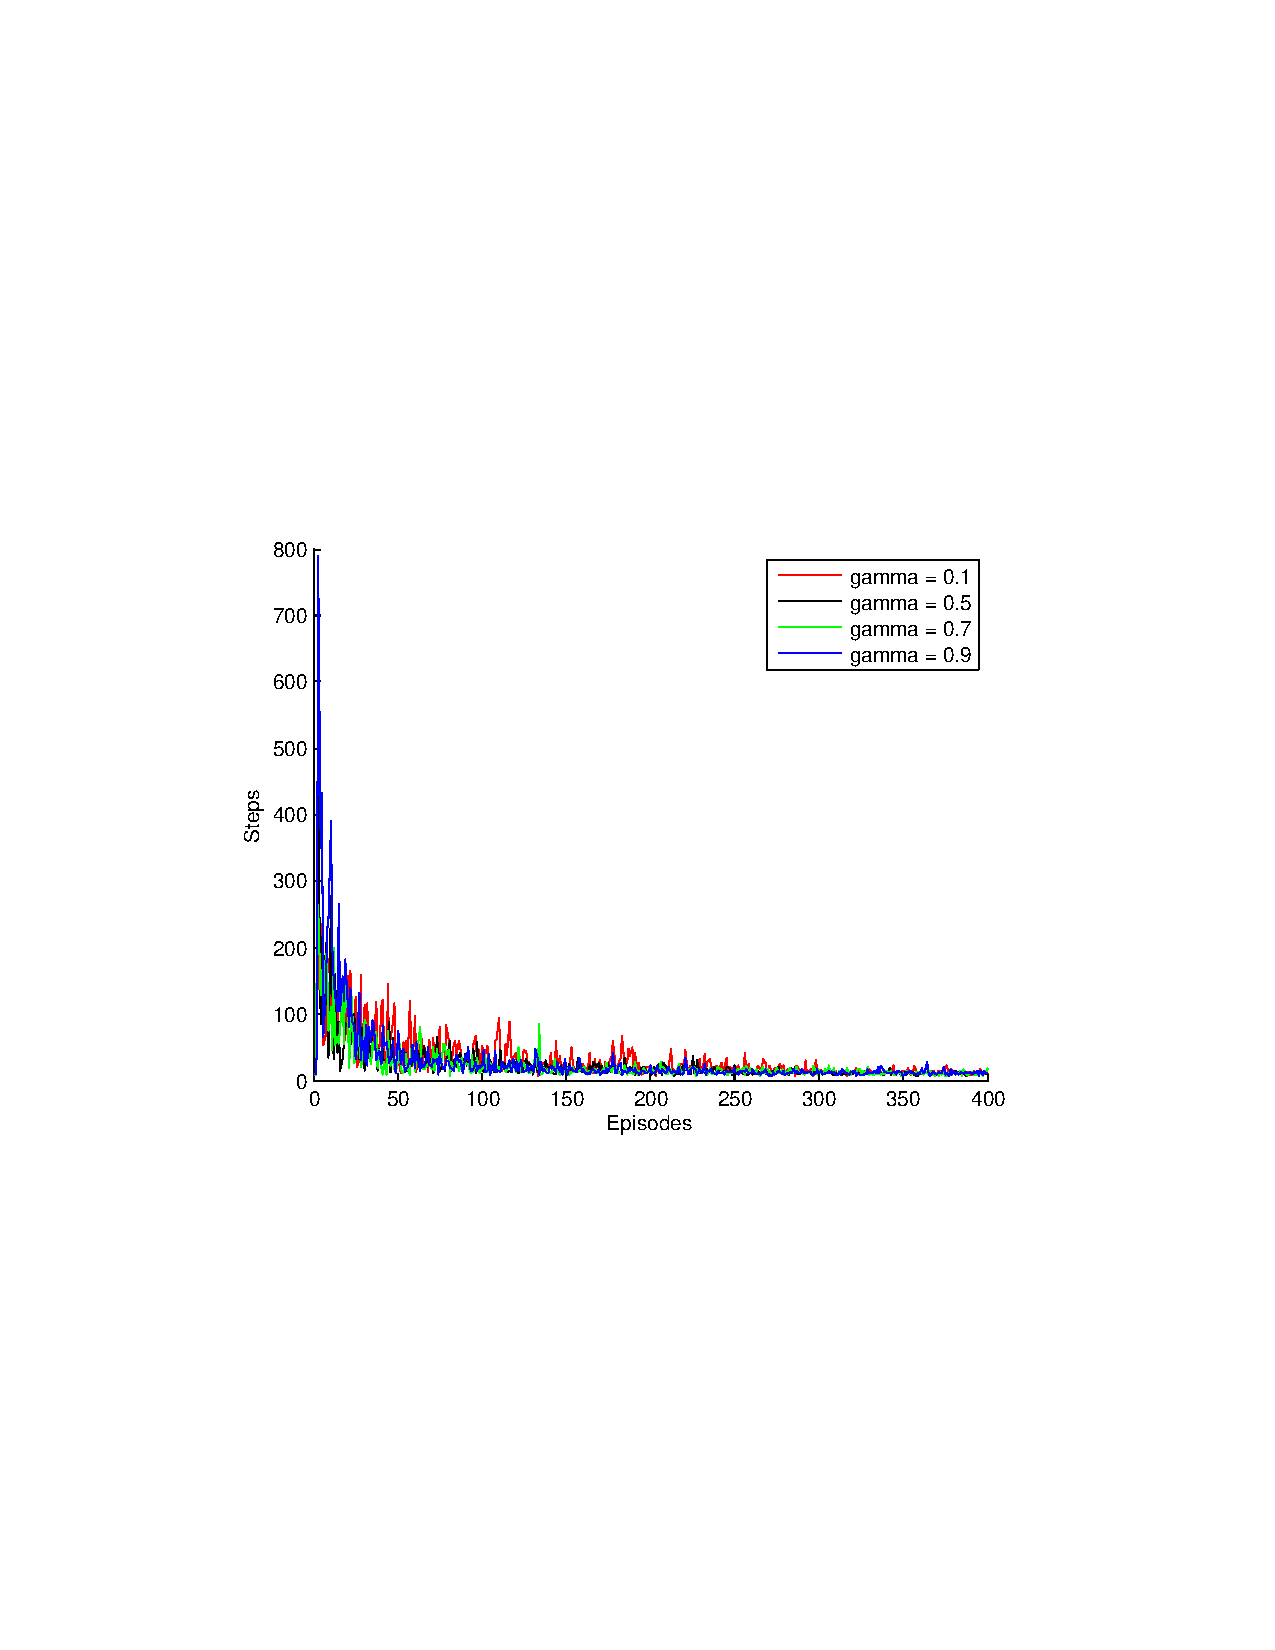
\includegraphics[trim=4cm 8.5cm 4cm 8.5cm,clip,width=0.75\textwidth]{figures/qla01.pdf}
    \caption{Q-learning results for different values of discount factor $\gamma$, having learning rate $\alpha = 0.1$.}
    \label{q01}
\end{figure}
~
\begin{figure}[h!]
  \centering
    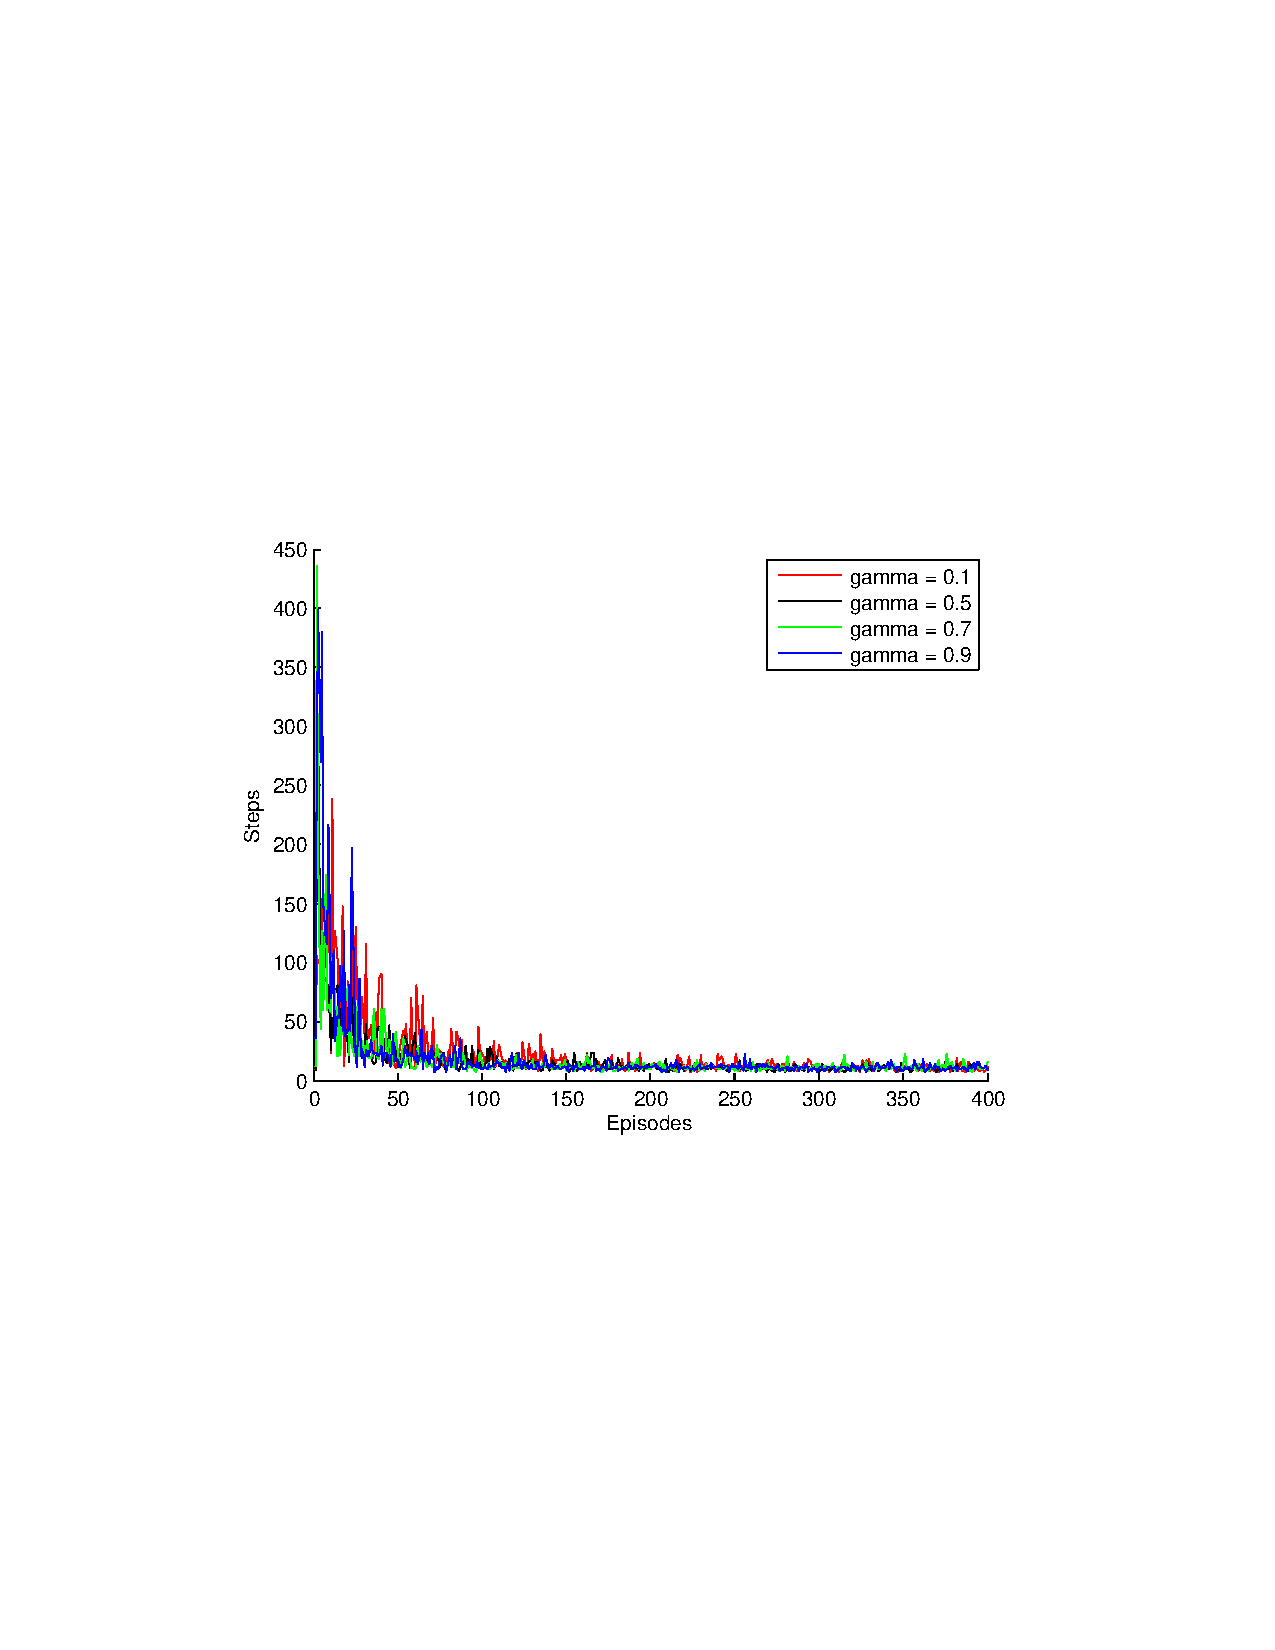
\includegraphics[trim=4cm 8.5cm 4cm 8.5cm,clip,width=0.75\textwidth]{figures/qla02.pdf}
    \caption{Q-learning results for different values of discount factor $\gamma$, having learning rate $\alpha = 0.2$.}
    \label{q02}
\end{figure}

\begin{figure}[h!]
  \centering
    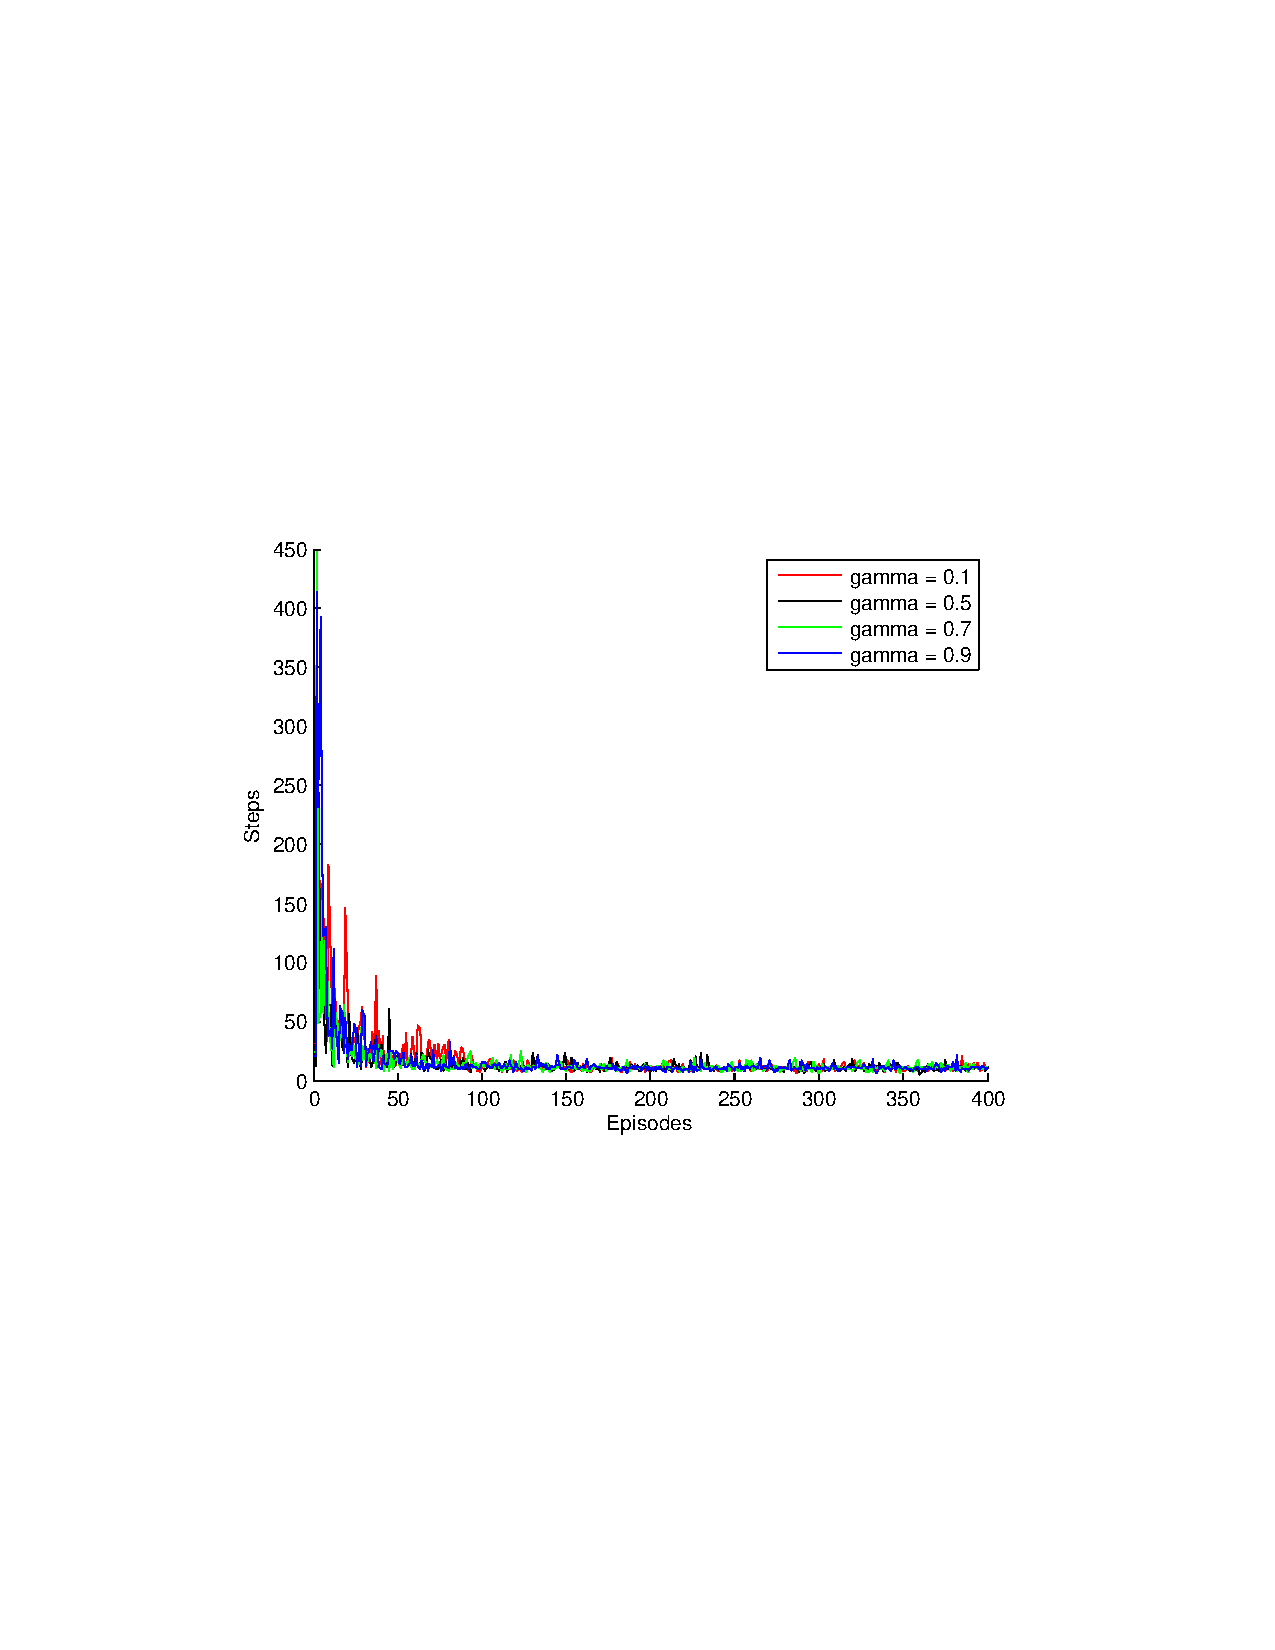
\includegraphics[trim=4cm 8.5cm 4cm 8.5cm,clip,width=0.75\textwidth]{figures/qla03.pdf}
    \caption{Q-learning results for different values of discount factor $\gamma$, having learning rate $\alpha = 0.3$.}
    \label{q03}
\end{figure}
~
\begin{figure}[h!]
  \centering
    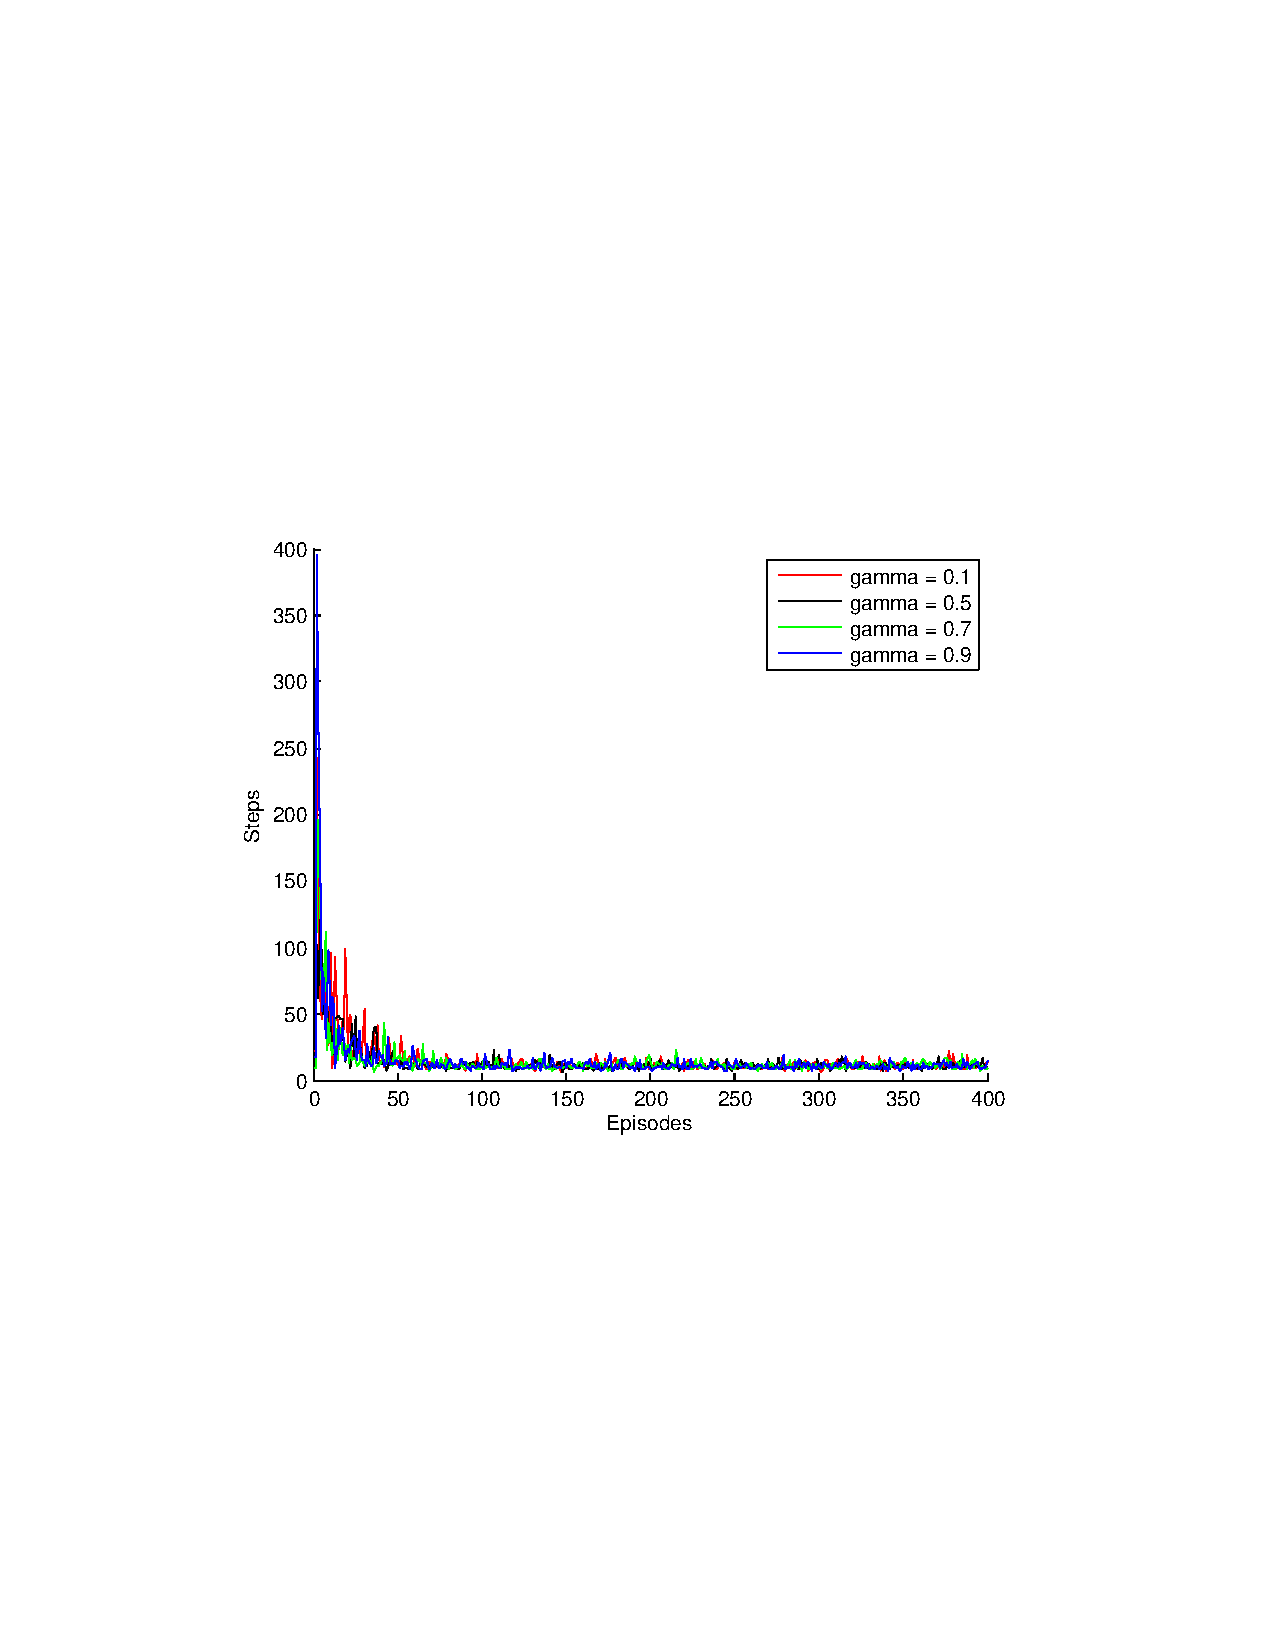
\includegraphics[trim=4cm 8.5cm 4cm 8.5cm,clip,width=0.75\textwidth]{figures/qla05.pdf}
    \caption{Q-learning results for different values of discount factor $\gamma$, having learning rate $\alpha = 0.5$.}
    \label{q05}
\end{figure}

Figures 1-4 clearly indicate how the predator learns faster while we increment the value of $\alpha$. Figure~\ref{q01} shows us that for $\alpha = 0.1$ the predator needs about 150 episodes to converge to the optimal ($\epsilon$-greedy) policy. However, while we increase alpha, the predator will need less episodes for the state-action pair values to converge. Increasing the value of $\alpha$ means that we consider the most recent information we observe, more important. A value of $\alpha = 0$ would mean that the predator is not learning at all, while $\alpha = 1$ means that the predator will overwrite the current value of the state-action pair with the new value, as can be easily seen:
\begin{align*}
  Q(s,a) &\leftarrow  Q(s,a) + 1 \left[ r + \gamma  \max_{a'} Q(s',a') - Q(s,a)\right] & \Longleftrightarrow\\
  Q(s,a) &\leftarrow  Q(s,a) - Q(s,a) + r + \gamma  \max_{a'} Q(s',a') & \Longleftrightarrow\\
  Q(s,a) &\leftarrow  r + \gamma  \max_{a'} Q(s',a') \\
\end{align*}
 
\section*{Exercise 2}

In this exercise we have implemented Q-learning with $\epsilon$ -greedy action decision for different values for $\epsilon$ , using different initial values for the state-action pairs each time. We have used 3 different values for the initialization of the values of the state-action pair: a pessimistic one (5), a realistic one (10) and an optimistic one (15), to see how the agent behaves for different values of $\epsilon$ in each case. On the pessimistic implementation, we expect the agent to converge to the optimal path really fast (given low values for $\epsilon$). On the other hand, the optimistic implementation will cause more of an exlporatory behavior.


Figure~\ref{qcomp}, shows our tests with $\epsilon$-greedy action selection for the optimistic, realistic and pessimistic initialization of the values of the state-action pairs. As shown, the pessimistic value helps the agent converge to the optimal path faster than the other initializations of the state-action values, while the optimistic value lets the agent explore a lot more before it converges. Using a pessimistic value to initialize the state-action values could lead the agent's policy into a local optimal, but not necessarily into a global optimal. In cases that there are three or more different rewards (in our example, we only have $0$ and $10$), an agent can only explore until it finds the locally optimal path to the state with the submaximal award. A higher value for the initialization would have lead this agent to explore the world better before its policy converge to a locally optimal policy. 



\begin{figure}[t!]
  \centering
    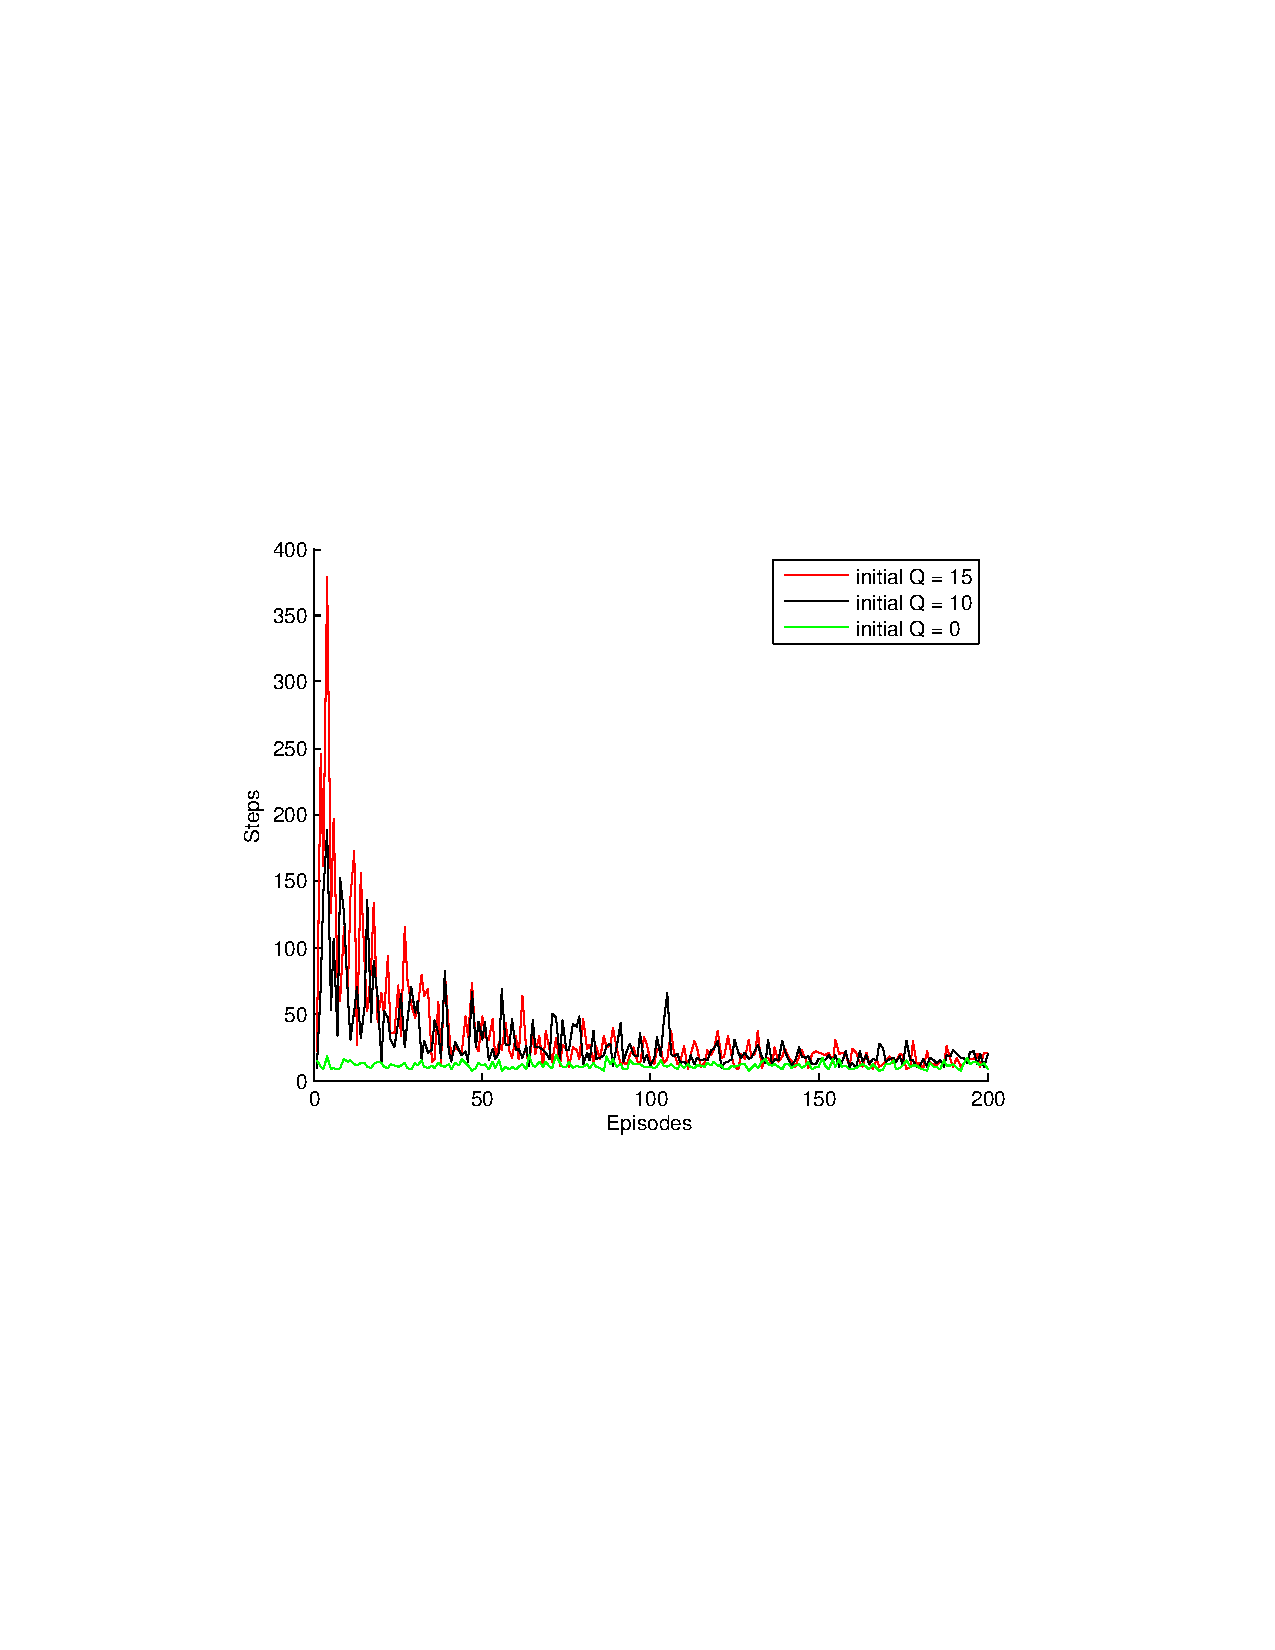
\includegraphics[trim=4cm 8.5cm 4cm 8.5cm,clip,width=0.75\textwidth]{figures/qcomp.pdf}
    \caption{Comparing implementations for different values for $Q_{initial}$  with $\alpha = 0.1$ , $\gamma=0.7$ .}
    \label{qcomp}
\end{figure}



We have chosen particular values for $\epsilon$ to test how, and what the predator will learn to do. For $\epsilon = 0$, the predator will always choose the action with the maximum value given the current state. Thus, the agent will converge to the optimal path really fast if the initial values of the state-action pairs are lower than any immediate reward, but it will become explorative if the state-action pair values are optimistically initialized.  This corresponds with a (deterministic) greedy policy.


If $\epsilon = 0.1$, the agent will try to exploit the action for which the Q-table has the maximum value with a probability of $1-\epsilon = 0.9$. That means that our predator is trying to exploit more than it is trying to explore, and there is a small probability that it will not choose the action it considers optimal.


\begin{figure}[t!]
  \centering
    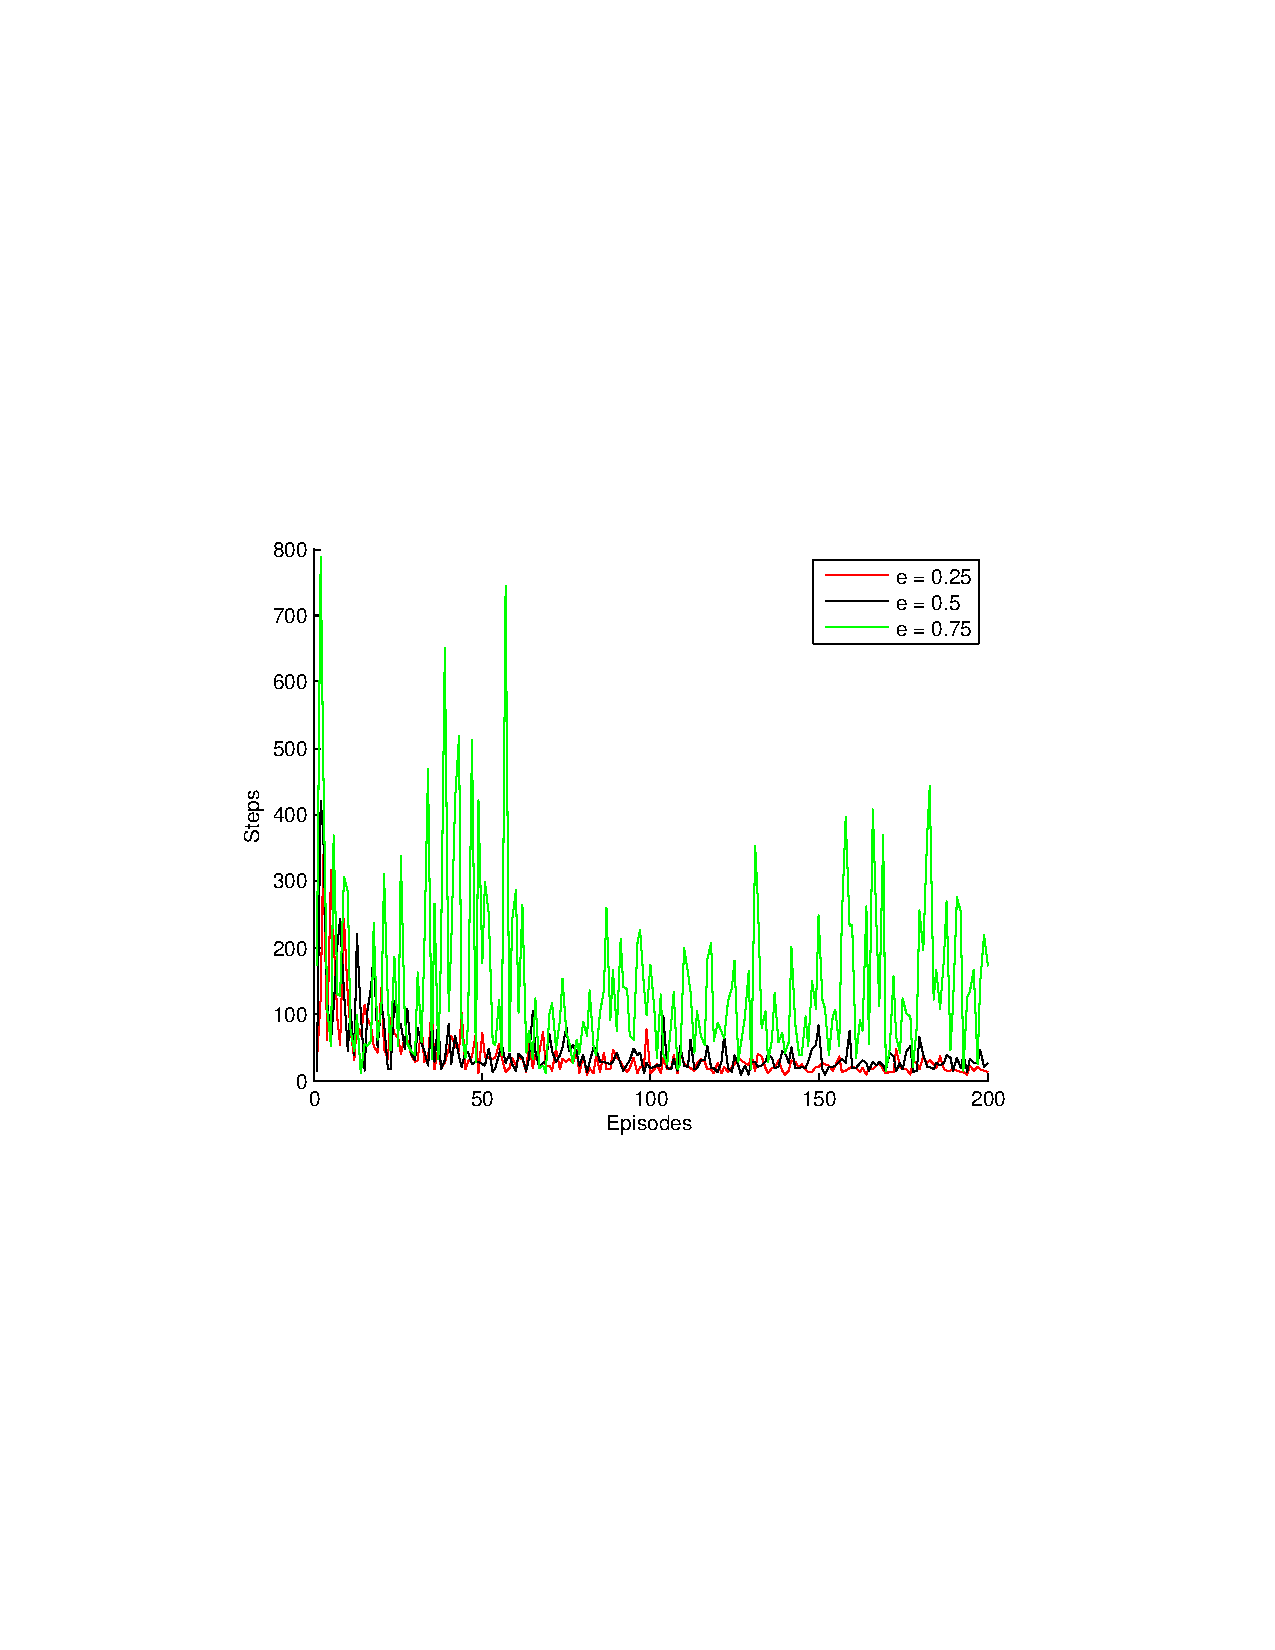
\includegraphics[trim=4cm 8.5cm 4cm 8.5cm,clip,width=0.7\textwidth]{figures/egreedycomp.pdf}
    \caption{Comparing different values of $\epsilon$ with $\epsilon$ -greedy action selection. For $\epsilon = 0.75$, the agent will be deciding its actions almost randomly.}
    \label{egreedycomp}
\end{figure}
~
\begin{figure}[h!]
  \centering
    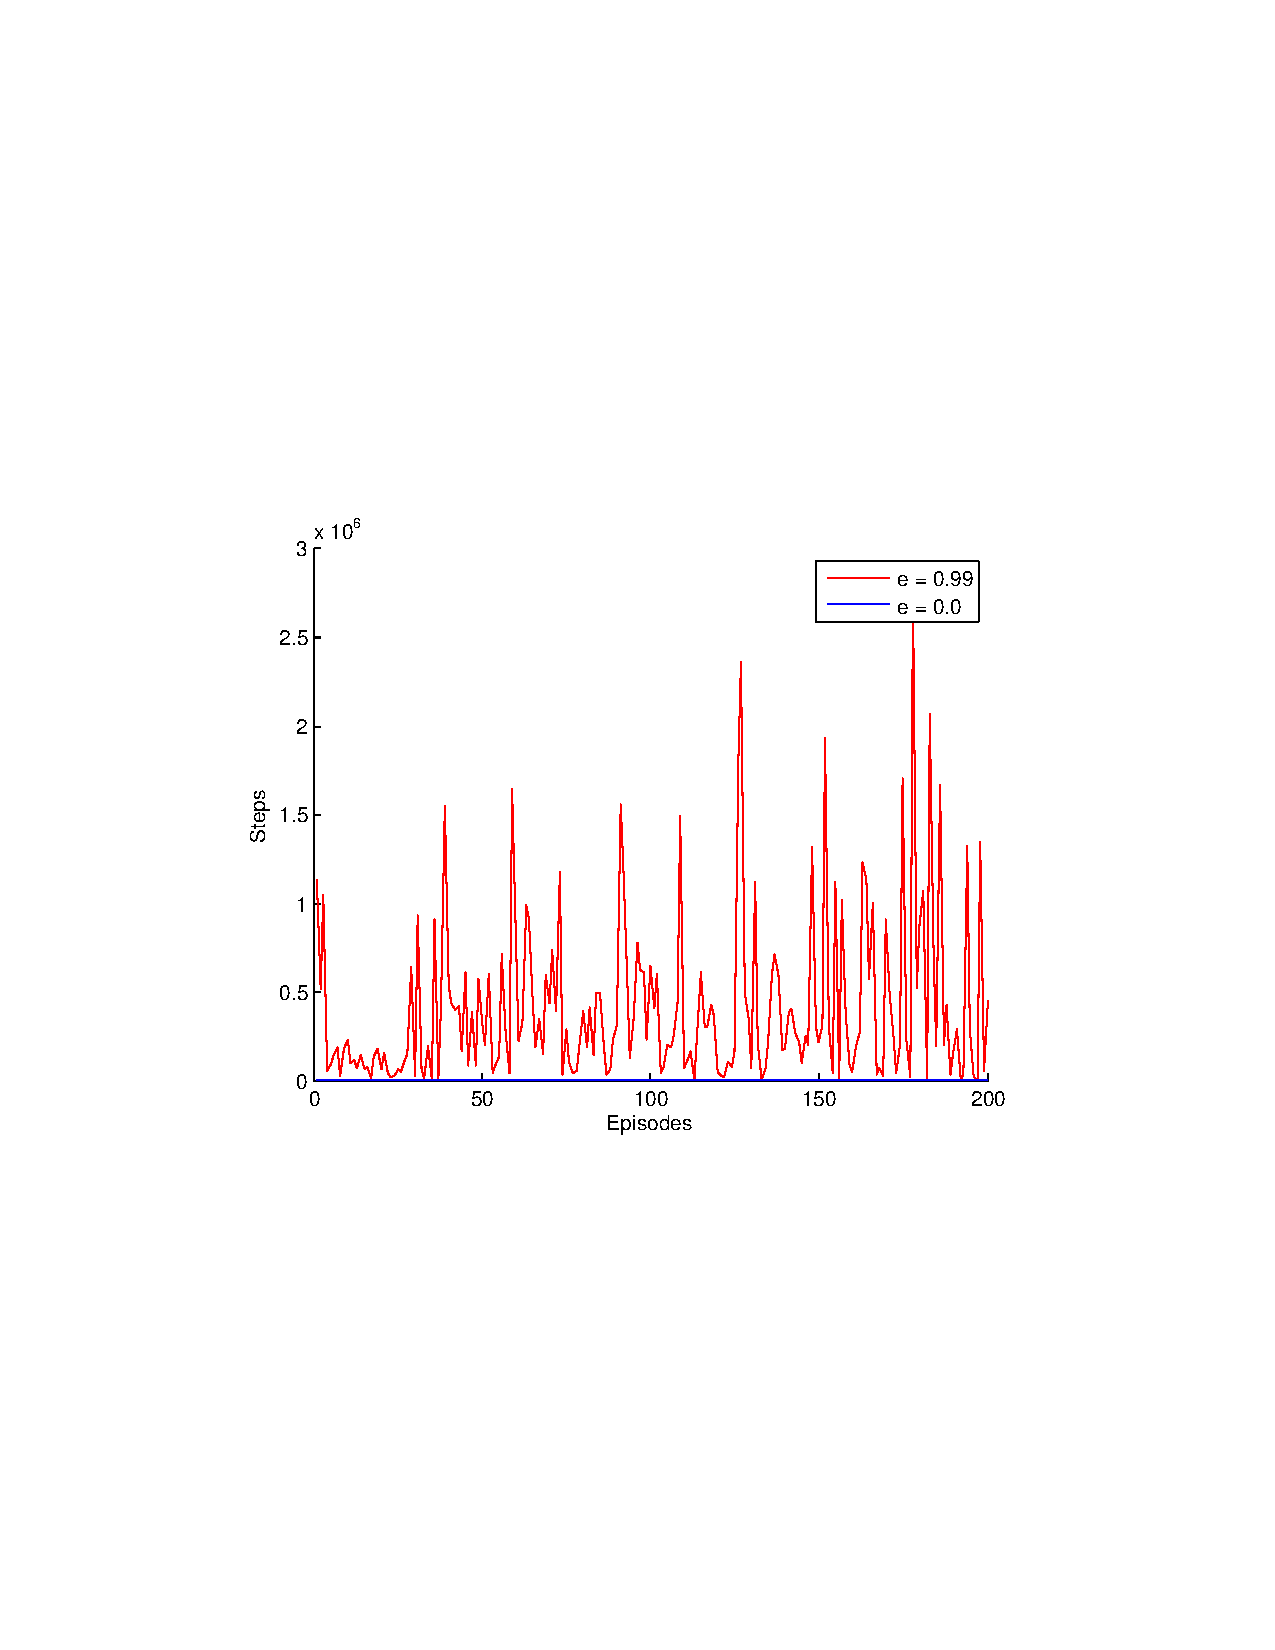
\includegraphics[trim=4cm 8.5cm 4cm 8.5cm,clip,width=0.7\textwidth]{figures/egreedyextreme.pdf}
    \caption{When the value of $\epsilon$ is close to $1$, the agent tends to avoid the maximum expected reward states.}
    \label{egreedyextreme}
\end{figure}

We have used the value of 0.8 for $\epsilon$ as well, because in this case, each possible action for the predator has the same probability to be chosen. Because the predator has 5 possible actions, there will be $1-\epsilon = 0.2$ probability for the optimal action to be chosen, and each of the other possible states will also have $\epsilon /4 = 0.2$ probability to be chosen. As a consequence, in the average case scenario our agent will be moving randomly. If there are less than 5 possible moves, he will be most likely be choosing one of the non-optimal moves.


Finally, we have also included $\epsilon = 0.99$ in our experimentation, for the reason that this value leaves $0.01$ probability for the agent to choose the optimal action. So, what happens in this case is that the predator learns not to use the optimal action each time he has to take a decision. As we see in the graphs, the number of steps it takes him to find the prey is increased dramatically as time goes by.


It should be pointed out that for initial values of the state-action pairs 10 and 15, the graphs are quite similar, with the plot of $\epsilon = 0.99$ dominating the other values. We only included this graph to show how this particular value of $\epsilon$ affects the behavior of the agent.





\section*{Exercise 3}

In this exercise we implemented softmax action selection besides $\epsilon$-greedy. 

Softmax differs from $\epsilon$-greedy in one important detail: $\epsilon$-greedy gives each non-optimal action a probability of $\epsilon$ divided by the number of non-optimal actions.  Softmax distributes weighted probability corresponding to the actions' values. This means, that in $\epsilon$-greedy the worst possible action has the same probability to be chosen as the second-to-best action, while in softmax, the worst possible action will typically have the lowest probability to be chosen.

Softmax chooses each action with probability equal to $\frac{e^{Q_t(a)/ \tau}}{\sum^n_{b=1} e^{Q_t(b)/ \tau}}$
where $\tau$ is a positive variable called ``temperature''. If $\tau \rightarrow \infty$ the possible actions tend to be equiprobable and thus corresponds to the random policy. However, if $\tau \rightarrow 0$, softmax tends to choose the next action greedily.

\begin{figure}[b!]
  \centering
    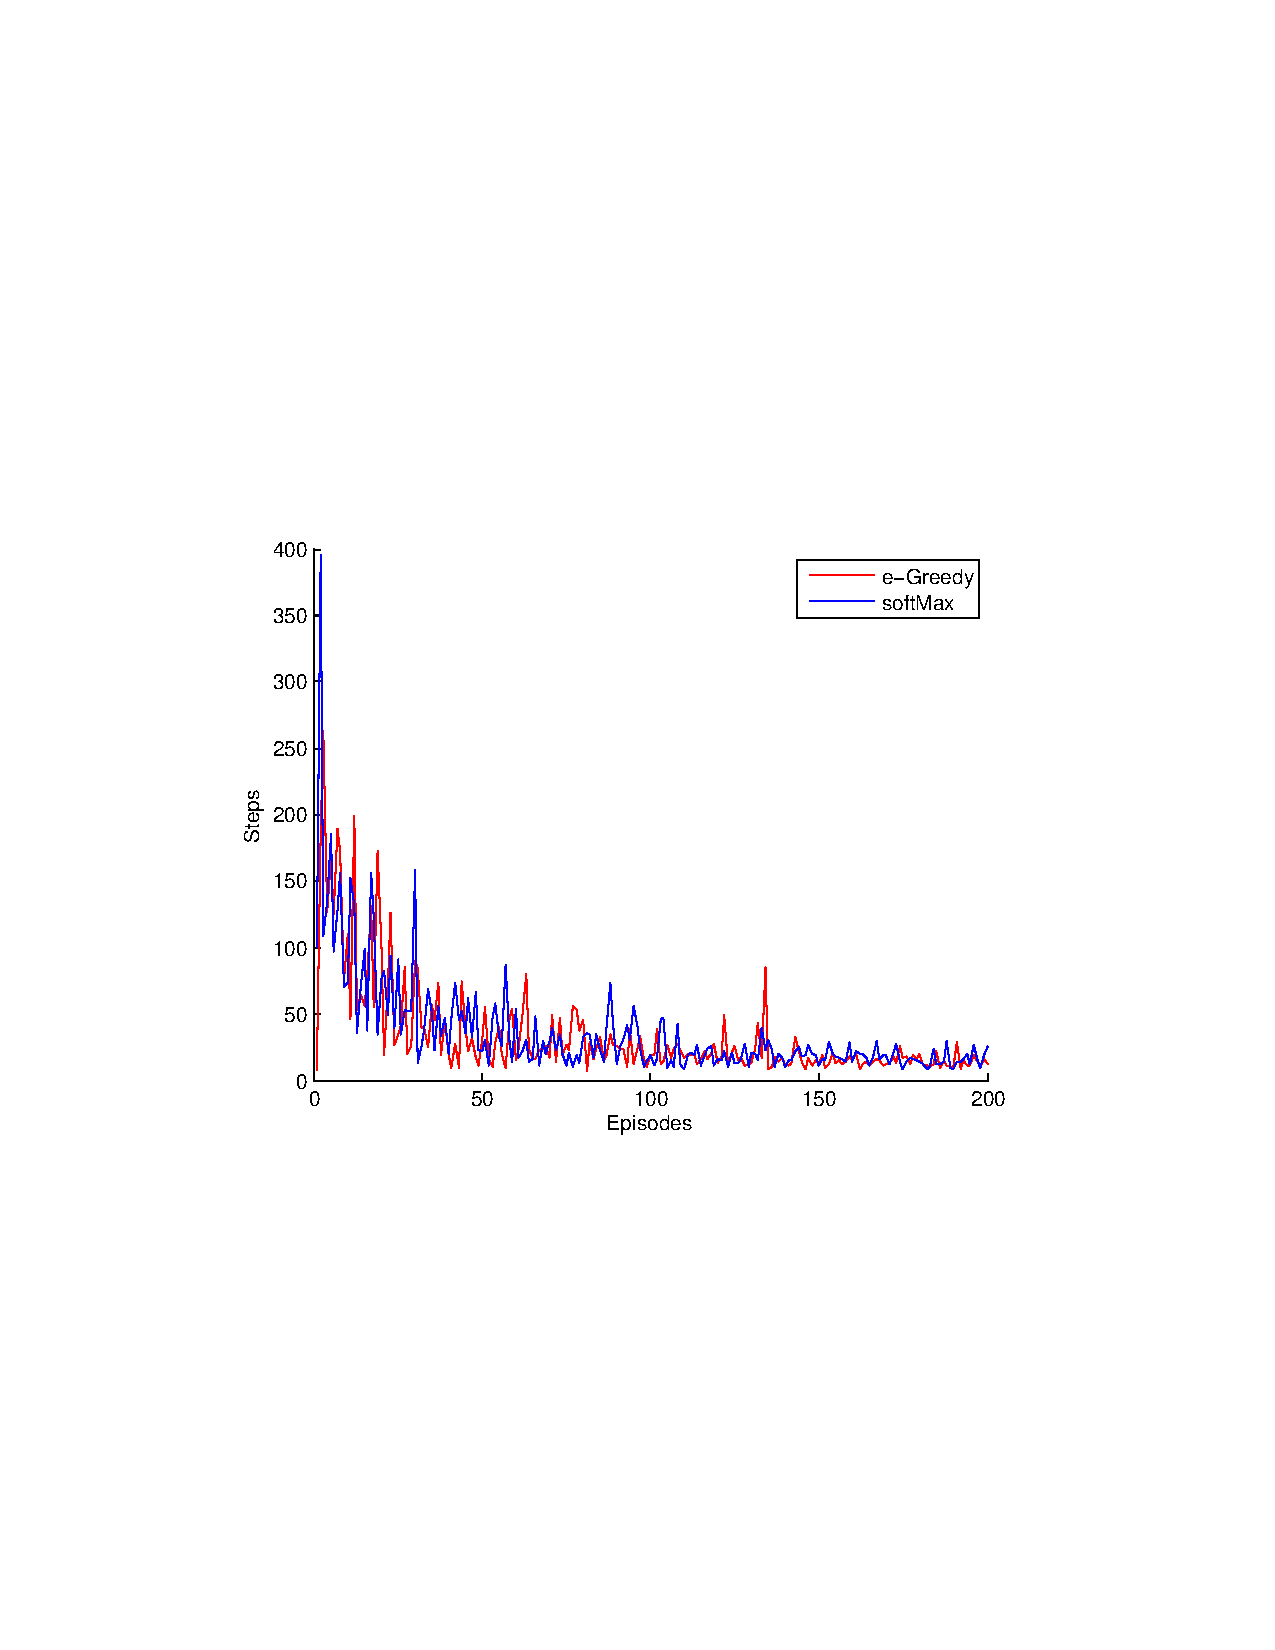
\includegraphics[trim=4cm 8.5cm 4cm 8.5cm,clip,width=0.6\textwidth]{figures/egresoftcomp.pdf}
    \caption{Comparing $\epsilon$-greedy and softmax implementations in Q-learning for $\alpha = 0.1$ , $\gamma = 0.7$, $\tau = 0.1$, $\epsilon = 0.1$ and $Q_{initial} = 15$.}
    \label{egresoftcomp}
\end{figure}

In our simulation, we found that $\epsilon$-greedy and softmax action selection are very much alike, and do not show any important difference. In figure 9, we have plotted the behavior of the agent with $\epsilon$-greedy and softmax implementation.













\section*{Exercise 4}
In the last exercise we went past the Q-learning algorithm and implemented the Sarsa, on-policy Monte Carlo and off-policy Monte Carlo algorithms. 	
\subsection*{Sarsa}
Sarsa is an on-policy temporal difference control method. On-policy TD methods use a certain policy (for example, $\epsilon$-greedy or softmax), which defines their future actions, and based on the reward they receive, they evaluate this policy.

On the other hand, off-policy TD methods do not ``stick'' to one particular policy, but can learn different policies and use the one for which they receive the best results. Another difference between on-policy and off-policy TD methods is that the latter update their value functions based on hypothetical actions, which actually they do not take, while on-policy TD methods are strictly based on the experience they gain from performing those actions.

\begin{figure}[t!]
  \centering
    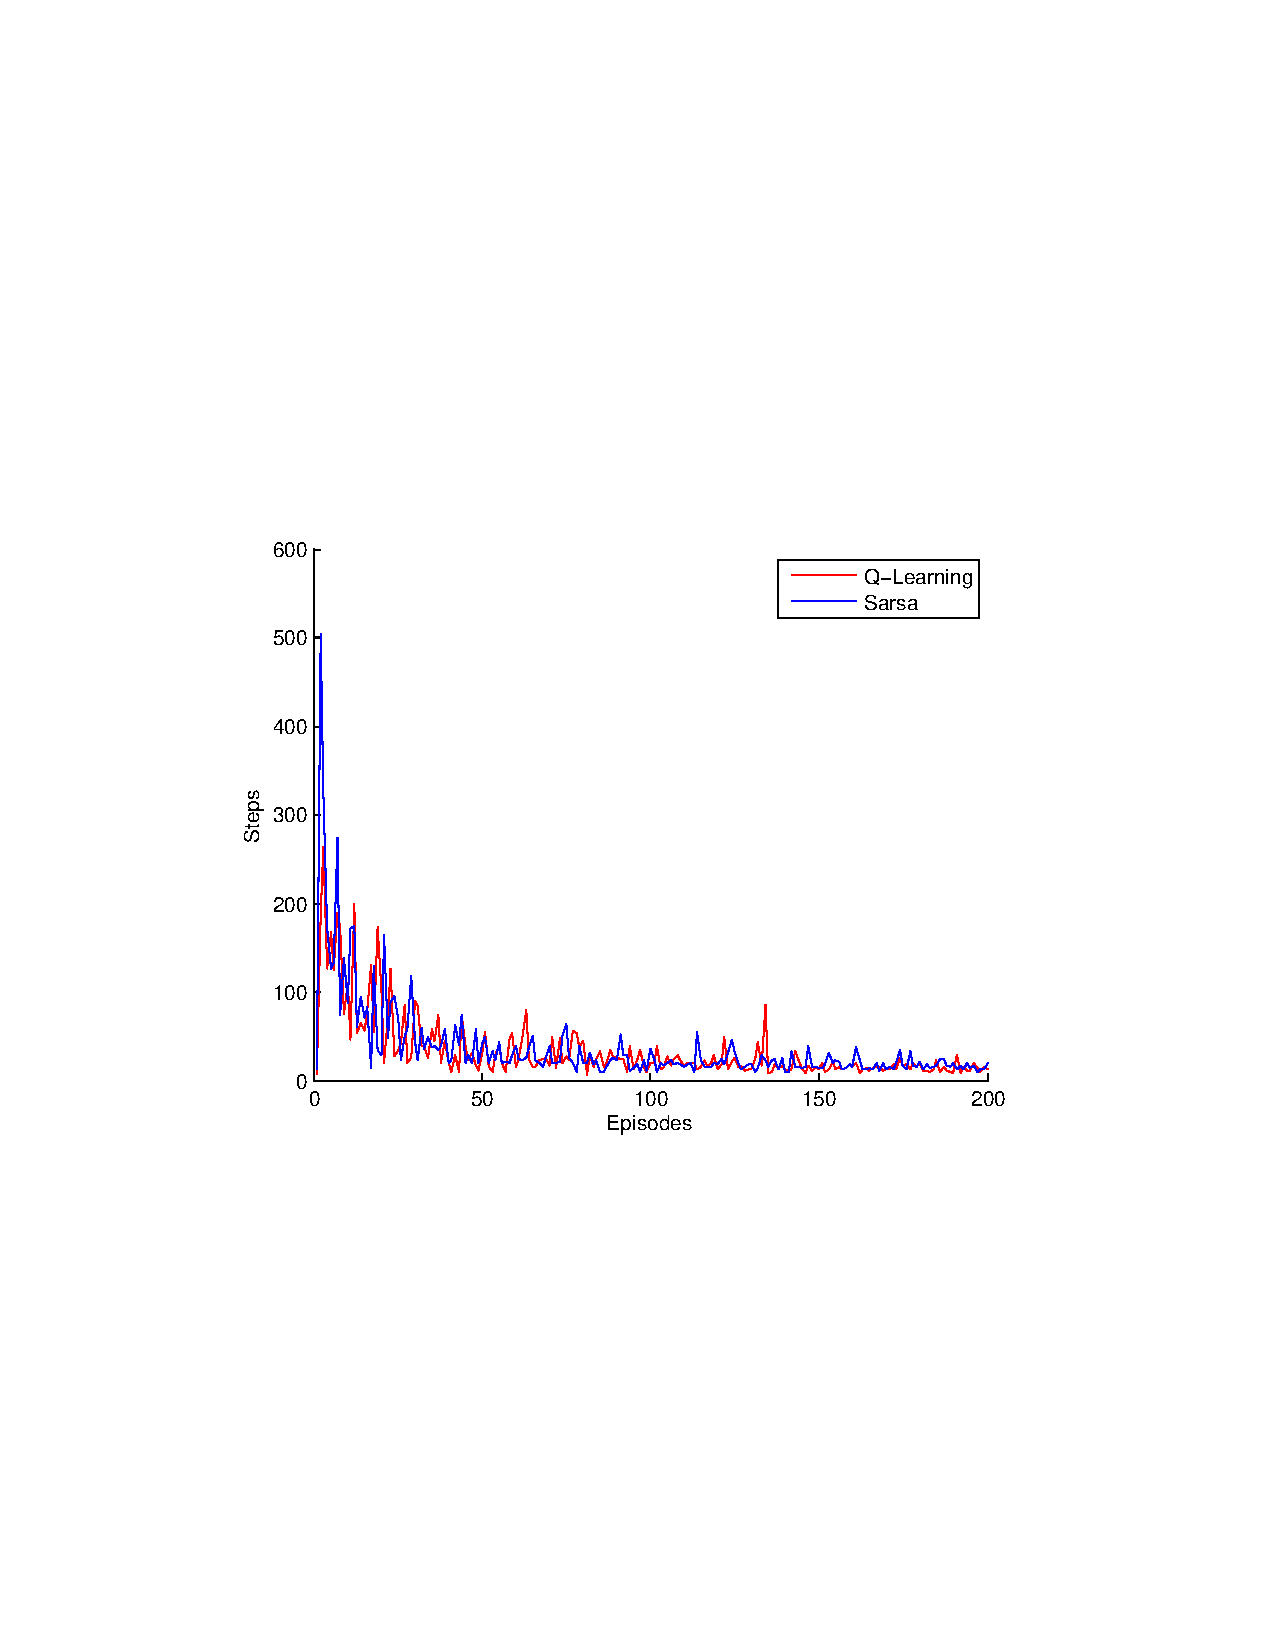
\includegraphics[trim=4cm 8.5cm 4cm 8.5cm,clip,width=0.75\textwidth]{figures/sarsaQcomp01.pdf}
    \caption{Comparing Sarsa and Q-learning algorithms for $\alpha = 0.1$, $\gamma = 0.7$ and $\epsilon = 0.1$.}
    \label{sarsaQcomp01}
\end{figure}

Sarsa and Q-learning have a lot in common, but there is an important difference that discriminates the two algorithms: When agent is at state $s$ and takes action $a$, Q-learning will update the Q table based on this action's reward. However, Sarsa will further observe the next state-action pair $(s',a')$ that derives from the next state $s'$ produced by action $a$. So, obviously, Sarsa needs two action selection steps, while Q-learning only needs one. Thus, Sarsa is considered an on-policy TD control method while Q-learning is considered to be off-policy.

On figure 10 we can look at a comparison between Q-learning and Sarsa algorithms' behavior. According to the graph, the two algorithms have quite similar results.

\begin{figure}[t!]
  \centering
    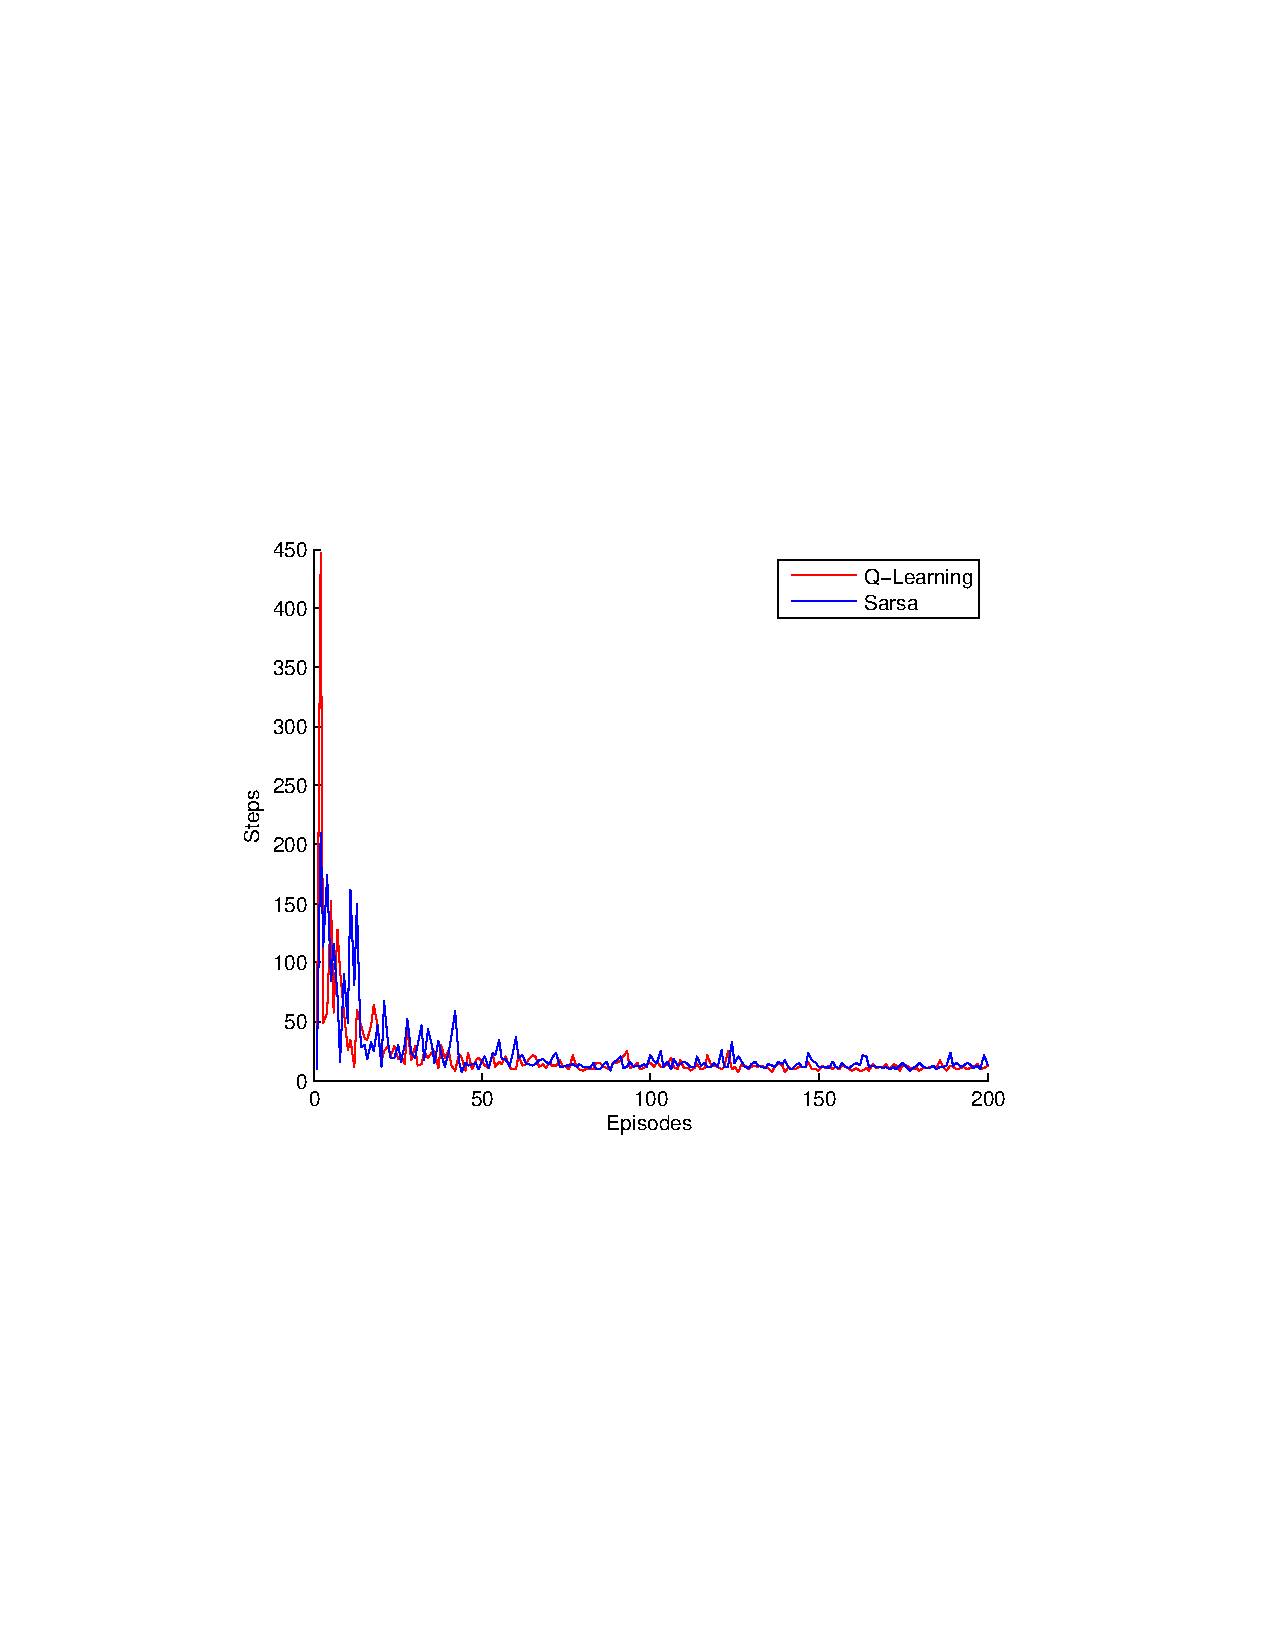
\includegraphics[trim=4cm 8.5cm 4cm 8.5cm,clip,width=0.75\textwidth]{figures/sarsaQcomp03.pdf}
    \caption{Comparing Sarsa and Q-learning algorithms for $\alpha = 0.3$, $\gamma = 0.7$ and $\epsilon = 0.1$.}
    \label{sarsaQcomp03}
\end{figure}



\subsection*{On-policy Monte Carlo}
Monte Carlo control methods come in on-policy and off-policy variants as well.  The
~
\begin{figure}[t!]
  \centering
    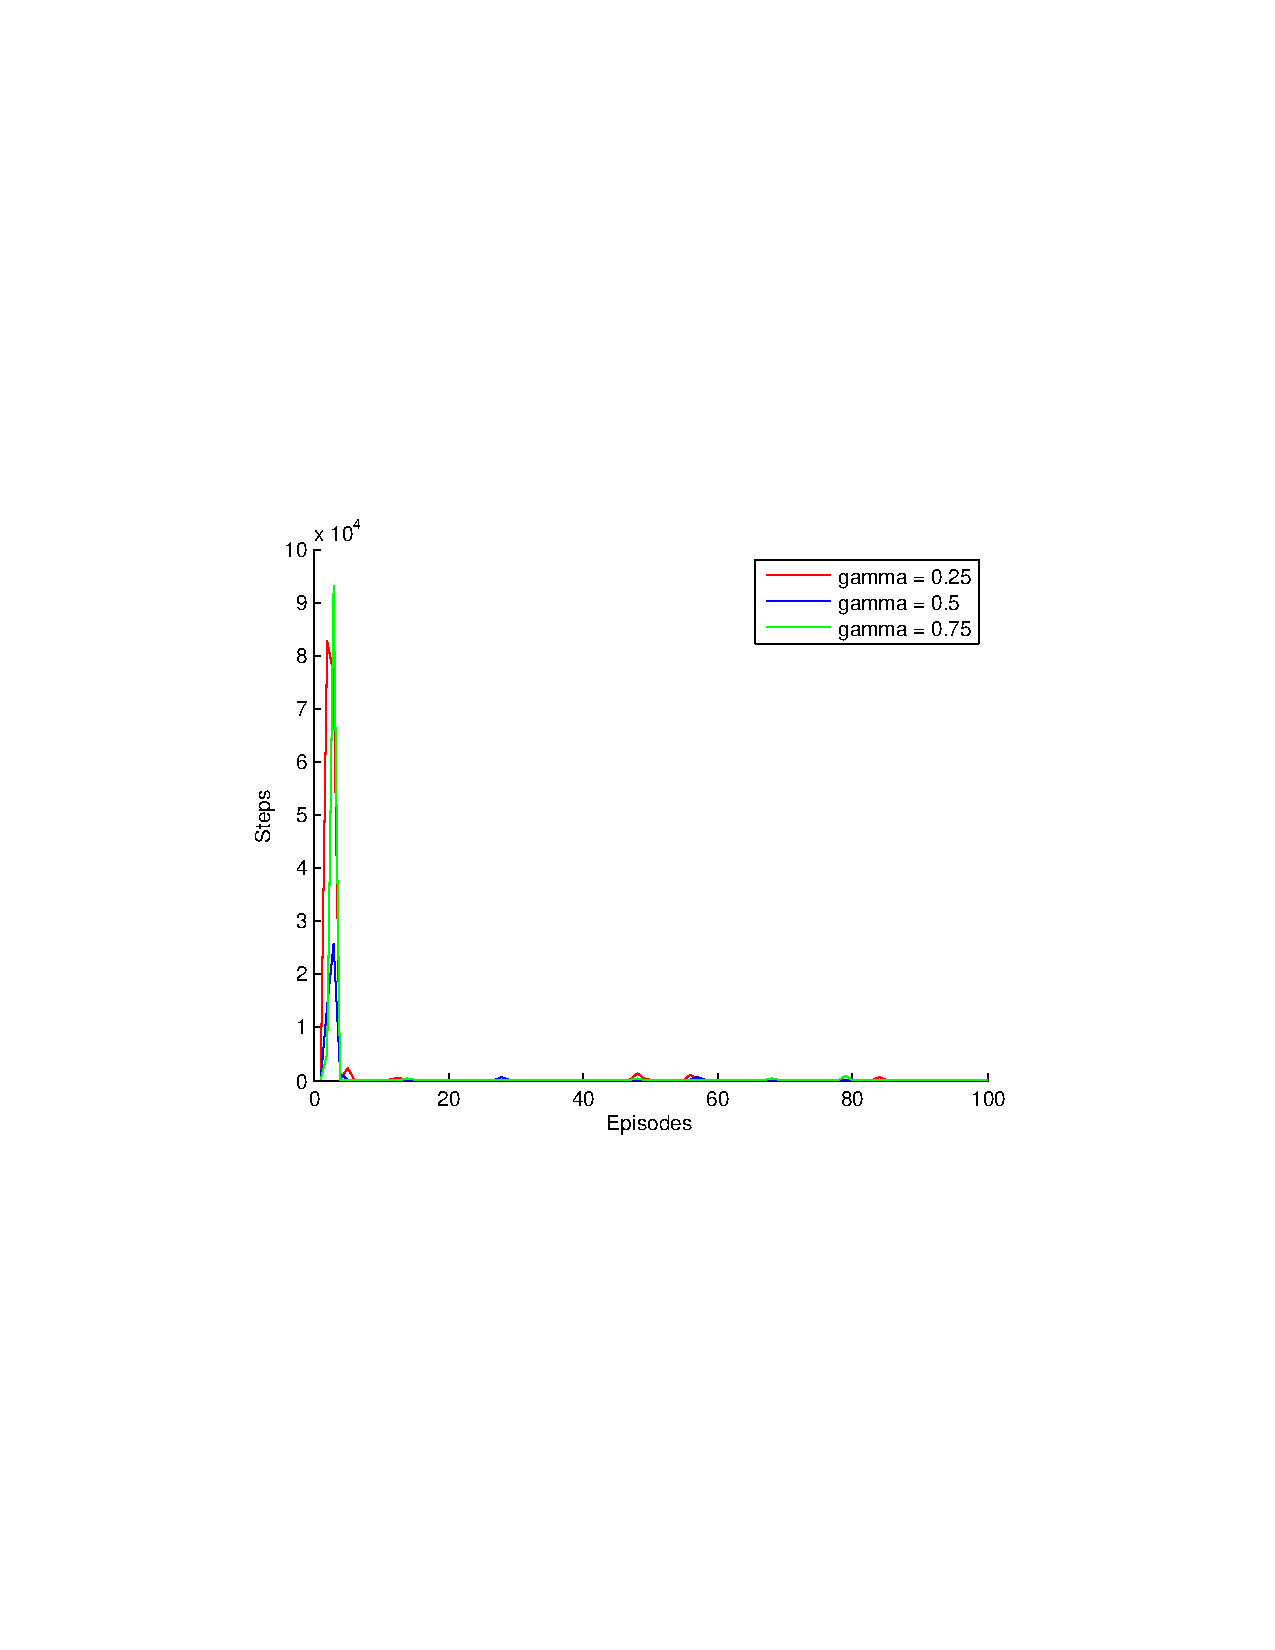
\includegraphics[trim=4cm 8.5cm 4cm 8.5cm,clip,width=0.75\textwidth]{figures/onmc.pdf}
    \caption{On-Policy Monte Carlo.}
     \label{onmc}
\end{figure}
\newpage


\subsection*{Off-policy Monte Carlo}
                                                                     
                                                                     
                                                                     
                                             
\section*{Off-policy Monte Carlo}
The Off-policy Monte Carlo control method is divided in 2 parts; the behavior function and the estimation function. The behavior function (or behavior policy) is the one used for the agent's learning, generating learning episodes which provide "knowledge" for the estimation policy to use later. The behavior policy is arbitrary, and the table that it creates is updated at the end of each episode, updating pairs of states and actions that agent used to find the prey. Consequentially, the predator's knowledge and its performance depend on the number of training episodes that the agent generates. First, we make use of e-greedy action selection policy to generate episodes. These episodes start always with the predator at (5,5), and prey at (0,0), and they end when the predator catches the prey. The behavior policy's Q table is computed as follows: 
\begin{enumerate}
\item the behavior policy generates an episode making use of the $\epsilon$ -greedy action selection policy.

\item starting from the end of each episode, we are finding the state $\tau$ in which was the last time where $a_\tau \neq \pi(s_\tau)$ where $\pi$ represents the behavior policy.

\item For each state-action pair appearing in the episode at time $\geq \tau$ from the first occurrence of $(s,a)$, $w \leftarrow \prod^{T-1}_{k=t+1}\frac{1}{\pi '(s_k,a_k)}$, where $w$ is called "weight" and is used for importance sampling, computing how important the return of an action is.

\item $N(s,a) \rightarrow N(s,a) + wR_t$,  where $R_t$ represents the return of action $a$ at time t, weighted by $w$.

\item $D(s,a) \rightarrow D(s,a) + w$

\item $Q(s,a) \rightarrow \frac{N(s,a)}{D(s,a)}$
\end{enumerate}

Using e-greedy does not mean that the action selection policy selects more optimal actions than a random approach. This happens because behavior policy depends on the Q-Table  which was initialized with equivalent values for all state action pairs. This was the learning part of this algorithm. It is obvious that it depends a lot on the action selection policy to update the values of each state action pair that exists in the world-state. Throughout the learning process and for small number of episodes, might be non-visited state action pairs. For this reason, a good selection policy, as well as, a large number of episodes have to be exist in order for this learning algorithm to converge into an optimal policy.

The estimation policy $\pi$ will use $argmax_aQ(s,a)$ to compute the next action from state $s$, which brings us to the conclusion that the estimation policy is always choosing the next action greedily. As shown clearly in figure 11, the more the training episodes the behavior policy generates, the better results we get from the estimation policy. Figures~\ref{offmc500},~\ref{offmc1000}, and~\ref{offmc10000}, present how the estimation policy behaves for different discount factor ($\gamma$) values while choosing the next action $\epsilon$ -greedily for 500, 1000, and 10000 episodes respectively. Looking at these Figures, we can realize that for a small discount factor and a large number of episodes this algorithm converges to the optimal policy. In contrary, even with a large number of episodes predator tends to need more steps in order to catch the prey. This happens due to the fact that using a large discount factor, we gave the chance to the predator wait further for its reward. Figure~\ref{offmc10000}, presents the computed policy that leads predator to catch prey in a very small number of steps, implied the functionality of the Monte Carlo off-line learning algorithm. 


\begin{figure}[h!]
  \centering
    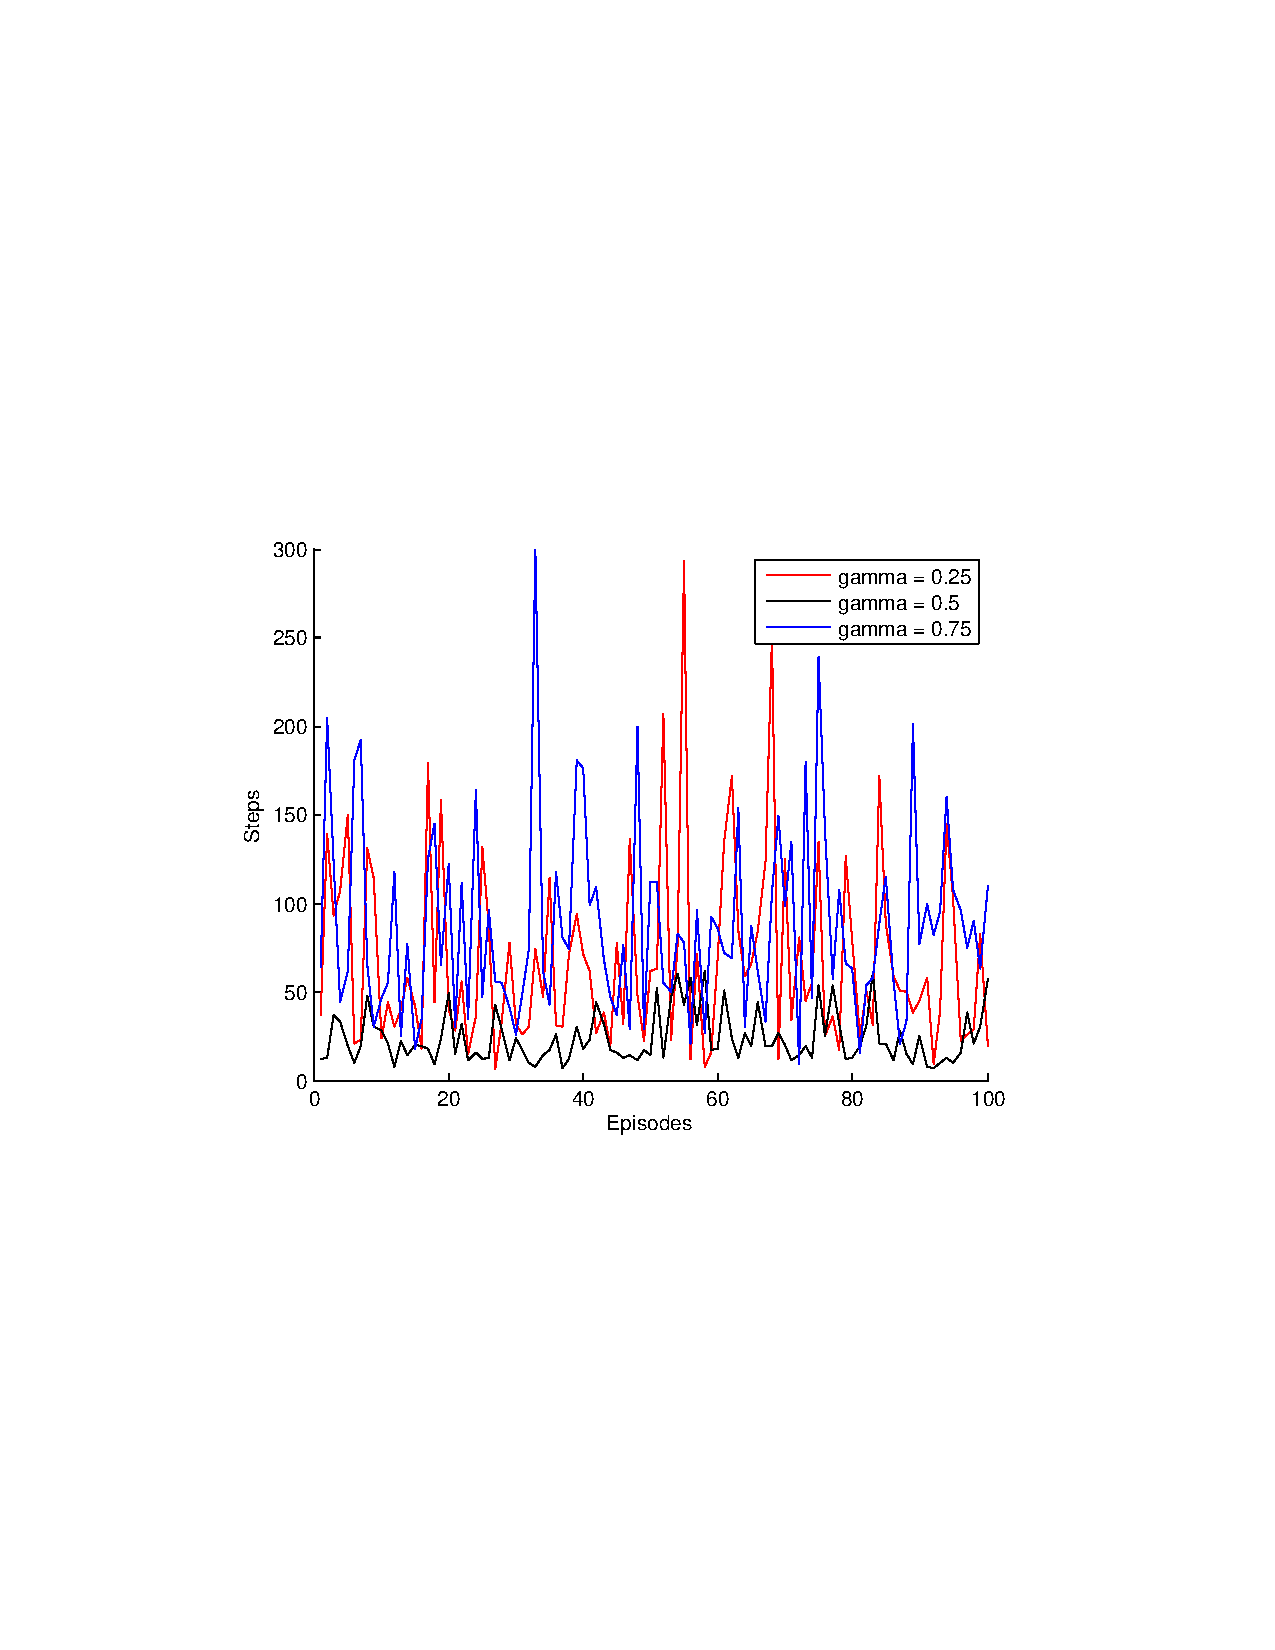
\includegraphics[trim=4cm 8.5cm 4cm 8.5cm,clip,width=0.75\textwidth]{figures/offmc500.pdf}
    \caption{Comparing Off-Policy Monte Carlo for 500 training episodes, with $\epsilon$ -greedy action selection ($\alpha = 0.2$, $\gamma = 0.7$).}
    \label{offmc500}
\end{figure}
~
\begin{figure}[h!]
  \centering
    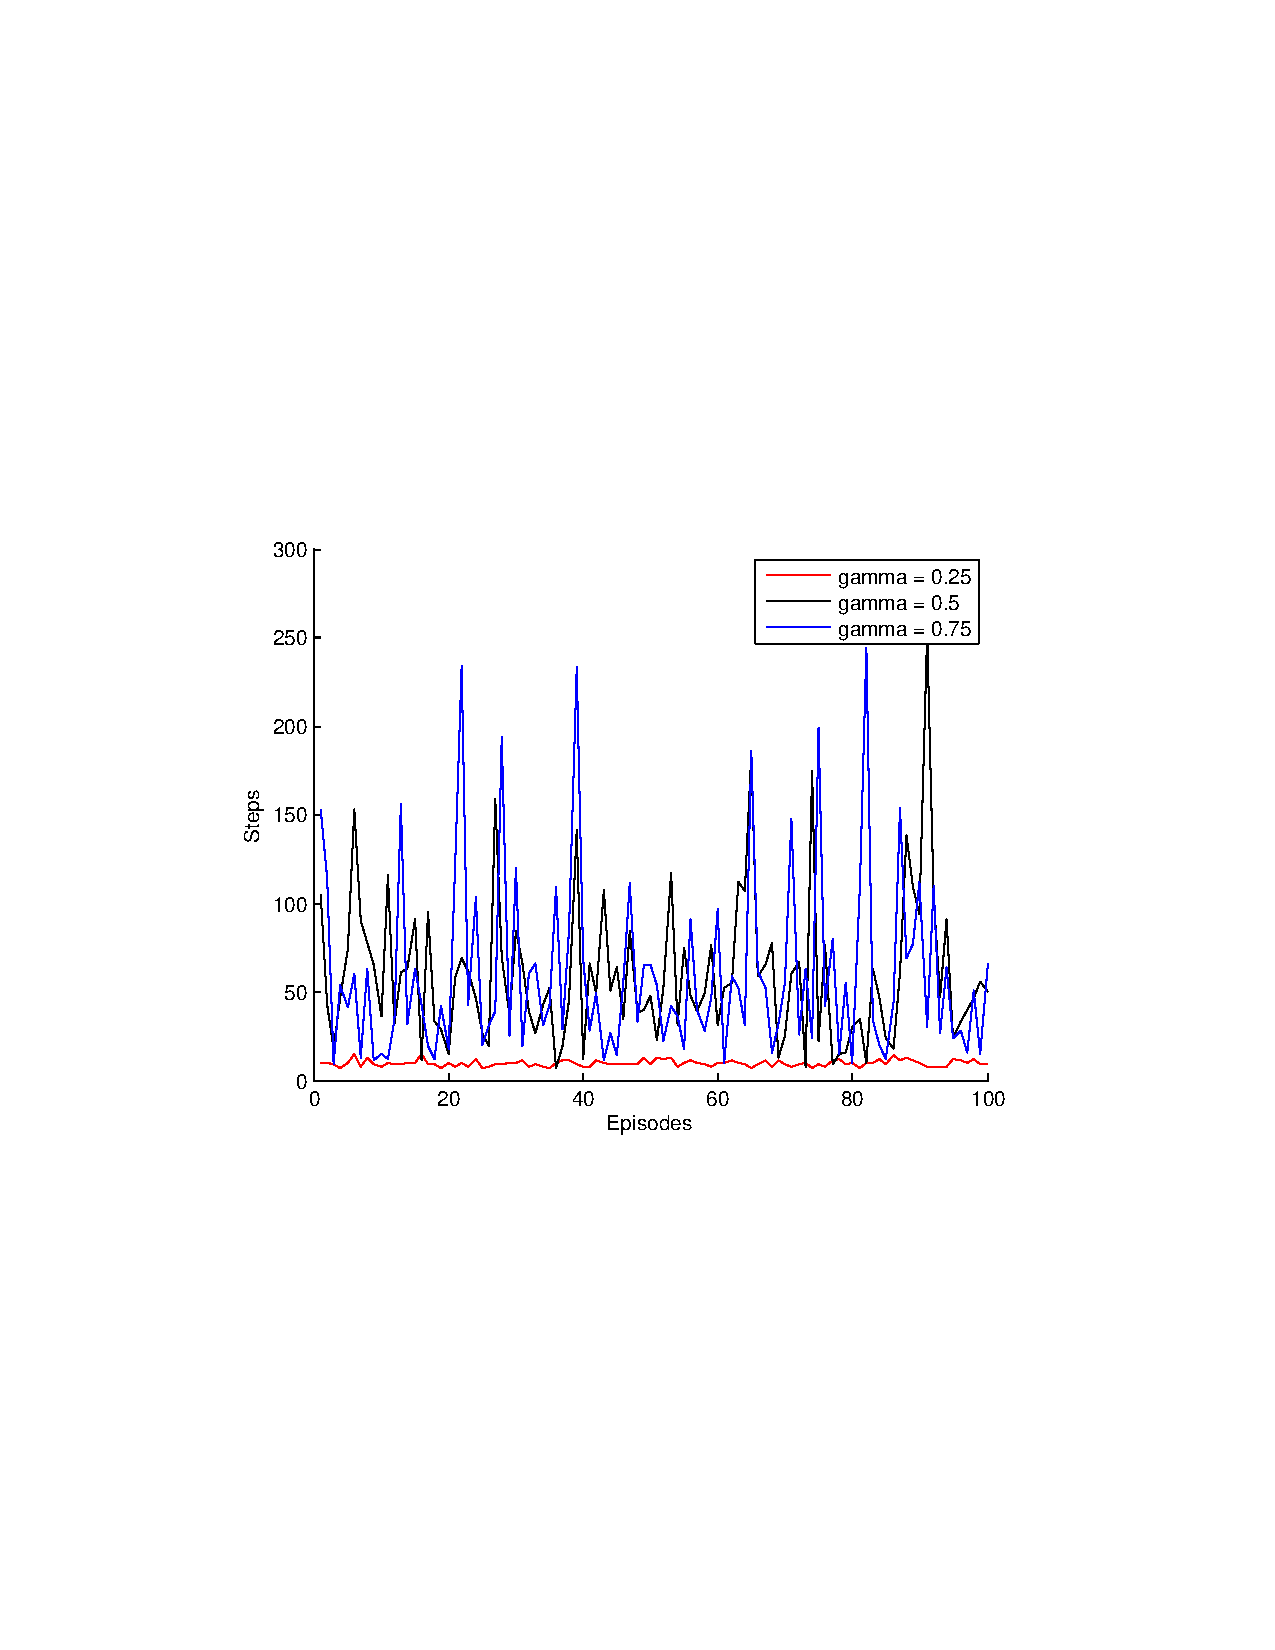
\includegraphics[trim=4cm 8.5cm 4cm 8.5cm,clip,width=0.75\textwidth]{figures/offmc1000.pdf}
    \caption{Comparing Off-Policy Monte Carlo for different values of $\gamma$, for 1000 training episodes.}
    \label{offmc1000}
\end{figure}
~
\begin{figure}[h!]
  \centering
    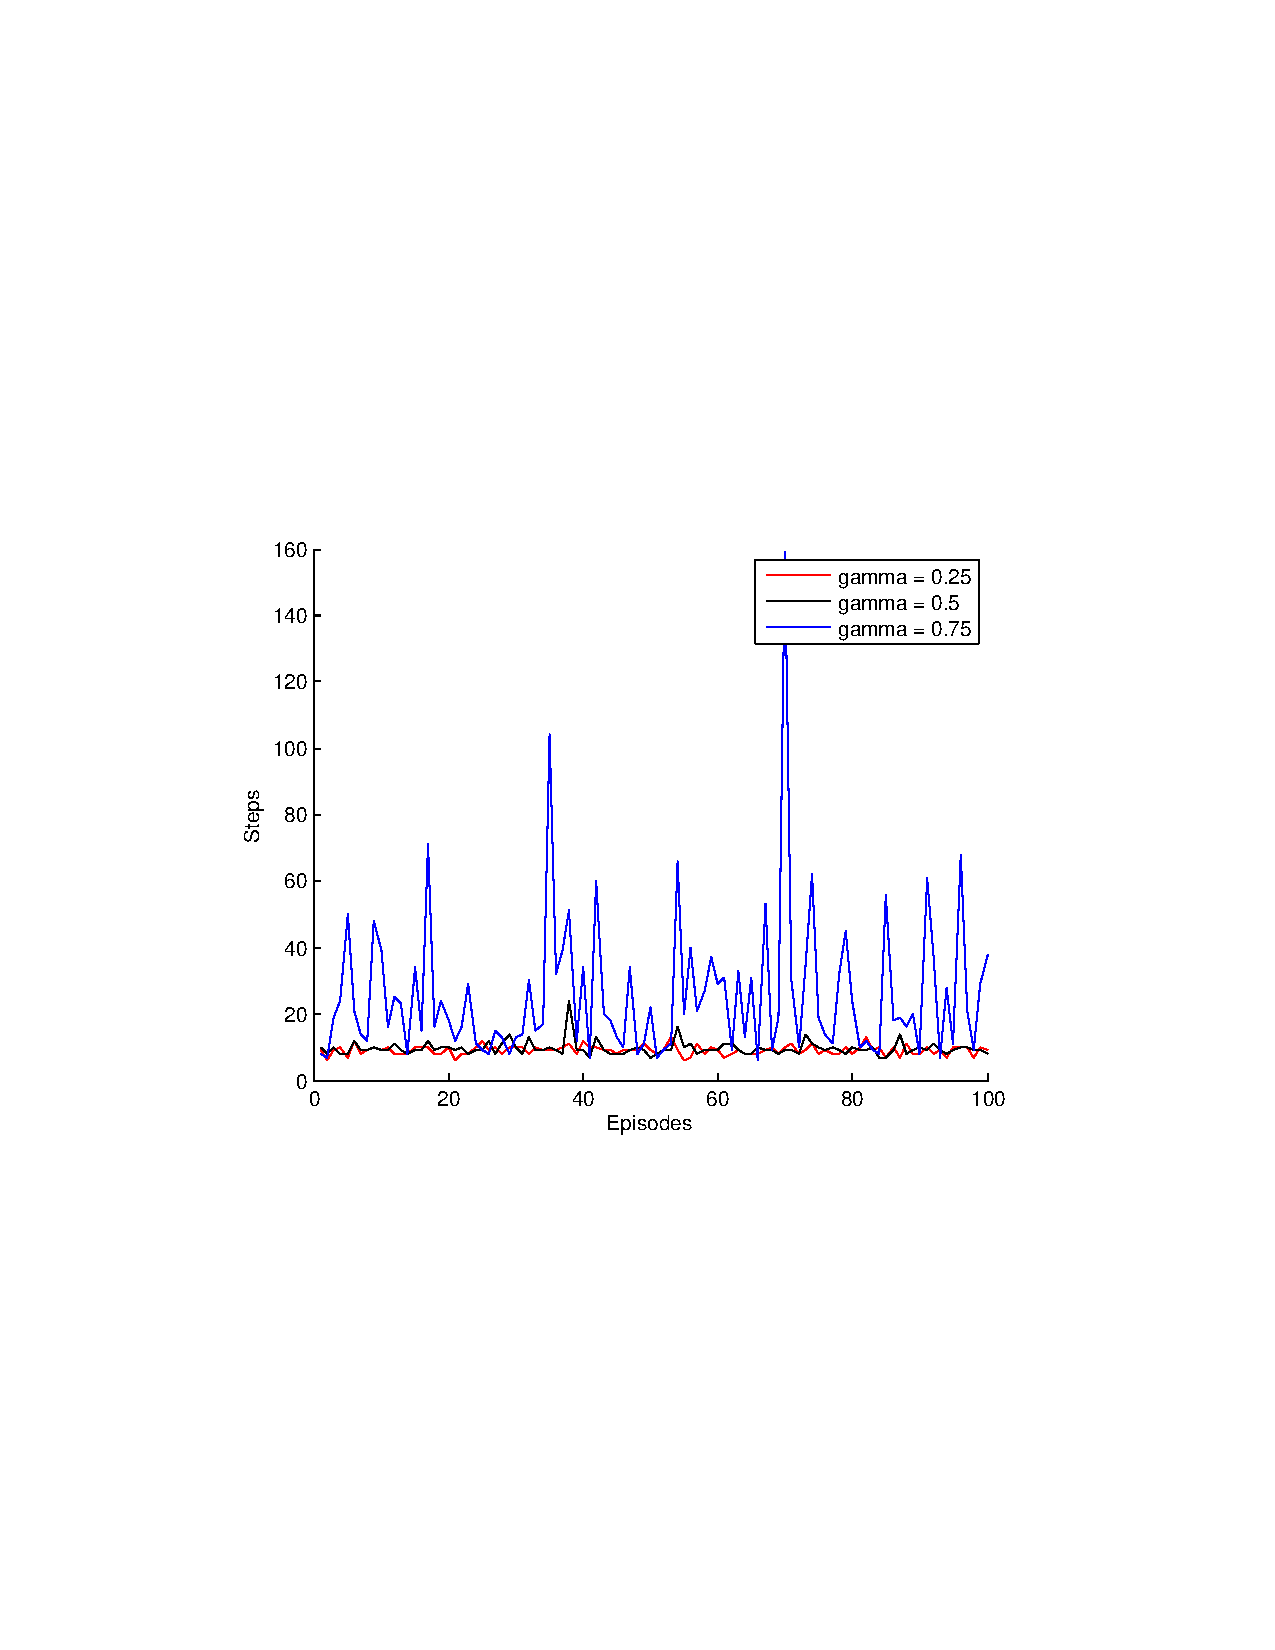
\includegraphics[trim=4cm 8.5cm 4cm 8.5cm,clip,width=0.75\textwidth]{figures/offmc10000.pdf}
    \caption{Comparing Off-Policy Monte Carlo for different values of $\gamma$, for 10000 training episodes.}
    \label{offmc10000}
\end{figure}

\newpage

\section*{Conclusion}

\end{document}

